\providecommand{\slides}{
  \newcommand{\slideshead}{
  \newcommand{\thepage}{\arabic{mypage}}
  %beamer
  \documentclass[t,hyperref={bookmarks=true}]{beamer}
%  \documentclass[t,hyperref={bookmarks=true},aspectratio=169]{beamer}
  \setbeamersize{text margin left=5mm}
  \setbeamersize{text margin right=5mm}
  \usetheme{default}
  \usefonttheme[onlymath]{serif}
  \setbeamertemplate{navigation symbols}{}
  \setbeamertemplate{itemize items}{{\color{black}$\bullet$}}

  \newwrite\keyfile

  %\usepackage{palatino}
  \stdpackages
  \usepackage{multimedia}

  %%% geometry/spacing issues
  %
  \definecolor{bluecol}{rgb}{0,0,.5}
  \definecolor{greencol}{rgb}{0,.6,0}
  %\renewcommand{\baselinestretch}{1.1}
  \renewcommand{\arraystretch}{1.2}
  \columnsep 0mm

  \columnseprule 0pt
  \parindent 0ex
  \parskip 0ex
  %\setlength{\itemparsep}{3ex}
  %\renewcommand{\labelitemi}{\rule[3pt]{10pt}{10pt}~}
  %\renewcommand{\labelenumi}{\textbf{(\arabic{enumi})}}
  \newcommand{\headerfont}{\helvetica{13}{1.5}{b}{n}}
  \newcommand{\slidefont} {\helvetica{10}{1.4}{m}{n}}
  \newcommand{\codefont} {\helvetica{8}{1.2}{m}{n}}
  \renewcommand{\small} {\helvetica{9}{1.4}{m}{n}}
  \renewcommand{\tiny} {\helvetica{8}{1.3}{m}{n}}
  \newcommand{\ttiny} {\helvetica{7}{1.3}{m}{n}}

  %%% count pages properly and put the page number in bottom right
  %
  \newcounter{mypage}
  \newcommand{\incpage}{\addtocounter{mypage}{1}\setcounter{page}{\arabic{mypage}}}
  \setcounter{mypage}{0}
  \resetcounteronoverlays{page}

  \pagestyle{fancy}
  %\setlength{\headsep}{10mm}
  %\addtolength{\footheight}{15mm}
  \renewcommand{\headrulewidth}{0pt} %1pt}
  \renewcommand{\footrulewidth}{0pt} %.5pt}
  \cfoot{}
  \rhead{}
  \lhead{}
%  \rfoot{{\tiny\textsf{AI -- \topic -- \subtopic -- \arabic{mypage}/\pageref{lastpage}}}}
%  \rfoot{\vspace*{-4.5mm}{\tiny\textsf{\topic\ -- \subtopic\ -- \arabic{mypage}/\pageref{lastpage}}}\hspace*{-4mm}}
  \rfoot{\vspace*{-4.5mm}{\tiny\textsf{\color{gray}\topic\ -- \subtopic\ -- \arabic{mypage}/\pageref{lastpage}}}\hspace*{-4mm}}
  %\lfoot{\raisebox{5mm}{\tiny\textsf{\slideauthor}}}
  %\rfoot{\raisebox{5mm}{\tiny\textsf{\slidevenue{} -- \arabic{mypage}/\pageref{lastpage}}}}
  %\rfoot{~\anchor{30,12}{\tiny\textsf{\thepage/\pageref{lastpage}}}}
  %\lfoot{\small\textsf{Marc Toussaint}}

  \definecolor{grey}{rgb}{.8,.8,.8}
  \definecolor{head}{rgb}{.85,.9,.9}
  \definecolor{blue}{rgb}{.0,.0,.5}
  \definecolor{green}{rgb}{.0,.5,.0}
  \definecolor{red}{rgb}{.8,.0,.0}
  \newcommand{\inverted}{
    \definecolor{main}{rgb}{1,1,1}
    \color{main}
    \pagecolor[rgb]{.3,.3,.3}
  }
  %auto-ignore
  \renewcommand{\a}{\alpha}
  \renewcommand{\b}{\beta}
  \renewcommand{\d}{\delta}
    \newcommand{\D}{\Delta}
    \newcommand{\e}{\epsilon}
    \newcommand{\g}{\gamma}
    \newcommand{\G}{\Gamma}
  \renewcommand{\l}{\lambda}
  \renewcommand{\L}{\Lambda}
    \newcommand{\m}{\mu}
    \newcommand{\n}{\nu}
    \newcommand{\N}{\nabla}
  \renewcommand{\k}{\kappa}
  \renewcommand{\o}{\omega}
  \renewcommand{\O}{\Omega}
    \newcommand{\p}{\phi}
    \newcommand{\ph}{\varphi}
  \renewcommand{\P}{\Phi}
  \renewcommand{\r}{\varrho}
    \newcommand{\s}{\sigma}
  \renewcommand{\S}{\Sigma}
  \renewcommand{\t}{\theta}
    \newcommand{\T}{\Theta}
  %\renewcommand{\v}{\vartheta}
    \newcommand{\x}{\xi}
    \newcommand{\X}{\Xi}
    \newcommand{\Y}{\Upsilon}
    \newcommand{\z}{\zeta}

  \renewcommand{\AA}{{\cal A}}
    \newcommand{\BB}{{\cal B}}
    \newcommand{\CC}{{\cal C}}
    \newcommand{\cc}{{\cal c}}
    \newcommand{\DD}{{\cal D}}
    \newcommand{\EE}{{\cal E}}
    \newcommand{\FF}{{\cal F}}
    \newcommand{\GG}{{\cal G}}
    \newcommand{\HH}{{\cal H}}
    \newcommand{\II}{{\cal I}}
    \newcommand{\KK}{{\cal K}}
    \newcommand{\LL}{{\cal L}}
    \newcommand{\MM}{{\cal M}}
    \newcommand{\NN}{{\cal N}}
    \newcommand{\oNN}{\overline\NN}
    \newcommand{\OO}{{\cal O}}
    \newcommand{\PP}{{\cal P}}
    \newcommand{\QQ}{{\cal Q}}
    \newcommand{\RR}{{\cal R}}
  \renewcommand{\SS}{{\cal S}}
    \newcommand{\TT}{{\cal T}}
    \newcommand{\uu}{{\cal u}}
    \newcommand{\UU}{{\cal U}}
    \newcommand{\VV}{{\cal V}}
    \newcommand{\XX}{{\cal X}}
    \newcommand{\xx}{\mathcal{x}}
    \newcommand{\YY}{{\cal Y}}
    \newcommand{\SOSO}{{\cal SO}}
    \newcommand{\GLGL}{{\cal GL}}

    \newcommand{\Ee}{{\rm E}}

  \newcommand{\NNN}{{\mathbb{N}}}
  \newcommand{\III}{{\mathbb{I}}}
  \newcommand{\ZZZ}{{\mathbb{Z}}}
  %\newcommand{\RRR}{{\mathrm{I\!R}}}
  \newcommand{\RRR}{{\mathbb{R}}}
  \newcommand{\SSS}{{\mathbb{S}}}
  \newcommand{\CCC}{{\mathbb{C}}}
  \newcommand{\DDD}{{\mathbb{D}}}
  \newcommand{\one}{{{\bf 1}}}
  \newcommand{\eee}{\text{e}}

  \newcommand{\NNNN}{{\overline{\cal N}}}

  \renewcommand{\[}{\Big[}
  \renewcommand{\]}{\Big]}
  \renewcommand{\(}{\Big(}
  \renewcommand{\)}{\Big)}
  \renewcommand{\|}{\,|\,}
  \renewcommand{\;}{\,;\,}
  \renewcommand{\=}{\!=\!}
    \newcommand{\<}{\left\langle}
  \renewcommand{\>}{\right\rangle}

  \newcommand{\na}[1][]{{\nabla_{\!\!#1}}}
  \newcommand{\he}[1][]{{\nabla_{\!\!#1}^2}}
  \newcommand{\Prob}{{\rm Prob}}
  \newcommand{\Dir}{{\rm Dir}}
  \newcommand{\Beta}{{\rm Beta}}
  \newcommand{\Bern}{{\rm Bern}}
  \newcommand{\Bin}{{\rm Bin}}
  \newcommand{\Mult}{{\rm Mult}}
  \newcommand{\Aut}{{\rm Aut}}
  \newcommand{\cor}{{\rm cor}}
  \newcommand{\corr}{{\rm corr}}
  \newcommand{\sd}{{\rm sd}}
  \newcommand{\tr}{{\rm tr}}
  \newcommand{\Tr}{{\rm Tr}}
  \newcommand{\rank}{{\rm rank}}
  \newcommand{\diag}{{\rm diag}}
  \newcommand{\dom}{{\rm dom}}
  \newcommand{\id}{{\rm id}}
  \newcommand{\Id}{{\rm\bf I}}
  \newcommand{\Gl}{{\rm Gl}}
  \renewcommand{\th}{\ensuremath{{}^\text{th}} }
  \newcommand{\lag}{\mathcal{L}}
  \newcommand{\inn}{\rfloor}
  \newcommand{\lie}{\pounds}
  \newcommand{\longto}{\longrightarrow}
  \newcommand{\speer}{\parbox{0.4ex}{\raisebox{0.8ex}{$\nearrow$}}}
  \renewcommand{\dag}{ {}^\dagger }
  \newcommand{\blbox}{\rule{1ex}{1ex}}
  \newcommand{\Ji}{J^\sharp}
  \newcommand{\h}{{}^\star}
  \newcommand{\w}{\wedge}
  \newcommand{\too}{\longrightarrow}
  \newcommand{\oot}{\longleftarrow}
  \newcommand{\To}{\Rightarrow}
  \newcommand{\oT}{\Leftarrow}
  \newcommand{\oTo}{\Leftrightarrow}
  \renewcommand{\iff}{~\Longleftrightarrow~}
  \newcommand{\Too}{\;\Longrightarrow\;}
  \newcommand{\oto}{\leftrightarrow}
  \newcommand{\ot}{\leftarrow}
  \newcommand{\ootoo}{\longleftrightarrow}
  \newcommand{\ow}{\stackrel{\circ}\wedge}
  \newcommand{\defeq}{\stackrel{\hspace{0.2ex}{}_\Delta}=}
%  \newcommand{\defeq}{{\overstack\Delta =}}
  \newcommand{\feed}{\nonumber \\}
  \newcommand{\comma}{~,\quad}
  \newcommand{\period}{~.\quad}
  \newcommand{\del}{\partial}
%  \newcommand{\quabla}{\Delta}
  \newcommand{\point}{$\bullet~~$}
  \newcommand{\doubletilde}{ ~ \raisebox{0.3ex}{$\widetilde {}$} \raisebox{0.6ex}{$\widetilde {}$} \!\! }
  \newcommand{\topcirc}{\parbox{0ex}{~\raisebox{2.5ex}{${}^\circ$}}}
  \newcommand{\topdot} {\parbox{0ex}{~\raisebox{2.5ex}{$\cdot$}}}
  \newcommand{\topddot} {\parbox{0ex}{~\raisebox{1.3ex}{$\ddot{~}$}}}
  \newcommand{\sym}{\topcirc}
  \newcommand{\tsum}{\textstyle\sum}
  \newcommand{\st}{\quad\text{s.t.}\quad}

  \newcommand{\half}{\ensuremath{\frac{1}{2}}}
  \newcommand{\third}{\ensuremath{\frac{1}{3}}}
  \newcommand{\fourth}{\ensuremath{\frac{1}{4}}}

  \newcommand{\ubar}{\underline}
  %\renewcommand{\vec}{\underline}
  \renewcommand{\vec}{\boldsymbol}
  %\renewcommand{\_}{\underset}
  %\renewcommand{\^}{\overset}
  %\renewcommand{\*}{{\rm\raisebox{-.6ex}{\text{*}}{}}}
  \renewcommand{\*}{\text{\footnotesize\raisebox{-.4ex}{*}{}}}

  \newcommand{\gto}{{\raisebox{.5ex}{${}_\rightarrow$}}}
  \newcommand{\gfrom}{{\raisebox{.5ex}{${}_\leftarrow$}}}
  \newcommand{\gnto}{{\raisebox{.5ex}{${}_\nrightarrow$}}}
  \newcommand{\gnfrom}{{\raisebox{.5ex}{${}_\nleftarrow$}}}

  %\newcommand{\RND}{{\SS}}
  %\newcommand{\IF}{\text{if }}
  %\newcommand{\AND}{\textsc{and }}
  %\newcommand{\OR}{\textsc{or }}
  %\newcommand{\XOR}{\textsc{xor }}
  %\newcommand{\NOT}{\textsc{not }}

  %\newcommand{\argmax}[1]{{\rm arg}\!\max_{#1}}
  %\newcommand{\argmin}[1]{{\rm arg}\!\min_{#1}}
  \DeclareMathOperator*{\argmax}{argmax}
  \DeclareMathOperator*{\argmin}{argmin}
  \DeclareMathOperator{\sign}{sign}
  \DeclareMathOperator{\acos}{acos}
  \DeclareMathOperator{\unifies}{unifies}
  \DeclareMathOperator{\Span}{span}
  \newcommand{\ortho}{\perp}
  %\newcommand{\argmax}[1]{\underset{~#1}{\text{argmax}}\;}
  %\newcommand{\argmin}[1]{\underset{~#1}{\text{argmin}}\;}
  \newcommand{\ee}[1]{\ensuremath{\cdot10^{#1}}}
  \newcommand{\sub}[1]{\ensuremath{_{\text{#1}}}}
  \newcommand{\up}[1]{\ensuremath{^{\text{#1}}}}
  \newcommand{\kld}[3][{}]{D_{#1}\big(#2\,\big|\!\big|\,#3\big)}
  %\newcommand{\kld}[2]{D\big(#1:#2\big)}
  \newcommand{\sprod}[2]{\big<#1\,,\,#2\big>}
  \newcommand{\End}{\text{End}}
  \newcommand{\txt}[1]{\quad\text{#1}\quad}
  \newcommand{\Over}[2]{\genfrac{}{}{0pt}{0}{#1}{#2}}
  %\newcommand{\mat}[1]{{\bf #1}}
  \newcommand{\arr}[2]{\hspace*{-.5ex}\begin{array}{#1}#2\end{array}\hspace*{-.5ex}}
  \newcommand{\mat}[3][.9]{
    \renewcommand{\arraystretch}{#1}{\scriptscriptstyle{\left(
      \hspace*{-1ex}\begin{array}{#2}#3\end{array}\hspace*{-1ex}
    \right)}}\renewcommand{\arraystretch}{1.2}
  }
  \newcommand{\Mat}[3][.9]{
    \renewcommand{\arraystretch}{#1}{\scriptscriptstyle{\left[
      \hspace*{-1ex}\begin{array}{#2}#3\end{array}\hspace*{-1ex}
    \right]}}\renewcommand{\arraystretch}{1.2}
  }
  \newcommand{\case}[2][ll]{\left\{\arr{#1}{#2}\right.}
  \newcommand{\seq}[1]{\textsf{\<#1\>}}
  \newcommand{\seqq}[1]{\textsf{#1}}
  \newcommand{\floor}[1]{\lfloor#1\rfloor}
  \newcommand{\Exp}[2][]{\text{E}_{#1}\{#2\}}
  \newcommand{\Var}[2][]{\text{Var}_{#1}\{#2\}}
  \newcommand{\cov}[2][]{\text{cov}_{#1}\{#2\}}

  %\newcommand{\Exp}[2]{\left\langle{#2}\right\rangle_{#1}}
  \newcommand{\ex}{\setminus}

  \providecommand{\href}[2]{{\color{blue}USE PDFLATEX!}}
  \providecommand{\url}[2]{\href{#1}{{\color{blue}#2}}}
%  \newcommand{\link}[1]{\href{{\protect #1}}{\texttt{\protect #1}}}
  \newcommand{\anchor}[2]{\begin{picture}(0,0)\put(#1){#2}\end{picture}}
  \newcommand{\pagebox}{\begin{picture}(0,0)\put(-3,-23){
    \textcolor[rgb]{.5,1,.5}{\framebox[\textwidth]{\rule[-\textheight]{0pt}{0pt}}}}
    \end{picture}}

  \newcommand{\hide}[1]{
    \begin{list}{}{\leftmargin0ex \rightmargin0ex \topsep0ex \parsep0ex}
       \helvetica{5}{1}{m}{n}
       \renewcommand{\section}{\par SECTION: }
       \renewcommand{\subsection}{\par SUBSECTION: }
       \item[$~~\blacktriangleright$]
       #1%$\blacktriangleleft~~$
       \message{^^JHIDE--Warning!^^J}
    \end{list}
  }
  %\newcommand{\hide}[1]{{\tt[hide:~}{\footnotesize\sf #1}{\tt]}\message{^^JHIDE--Warning!^^J}}
  \newcommand{\Hide}{\renewcommand{\hide}[1]{\message{^^JHIDE--Warning (hidden)!^^J}}}
  \newcommand{\HIDE}{\renewcommand{\hide}[1]{}}
  \newcommand{\fullhide}[1]{\message{^^JHIDE--Warning (hidden)!^^J}}
  \newcommand{\todo}[1]{{\tt[TODO: #1]}\message{^^JTODO--Warning: #1^^J}}
  \newcommand{\Todo}{\renewcommand{\todo}[1]{\message{^^JTODO--Warning (hidden)!^^J}}}
  %\renewcommand{\title}[1]{\renewcommand{\thetitle}{#1}}
  \newcommand{\myauthor}[1]{\author{#1}\newcommand{\theauthor}{#1}}%\@author}
  \newcommand{\mytitle}[1]{\title{#1}\newcommand{\thetitle}{#1}}%\@title}
  \newcommand{\header}{\begin{document}\mytitle\cleardefs}
  \newcommand{\contents}{{\tableofcontents}\renewcommand{\contents}{}}
  \newcommand{\footer}{\small\bibliography{marc,bibs}\end{document}}
  \newcommand{\widepaper}{\usepackage{geometry}\geometry{a4paper,hdivide={25mm,*,25mm},vdivide={25mm,*,25mm}}}
  \newcommand{\moviex}[2]{\movie[externalviewer]{#1}{#2}} %\pdflatex\usepackage{multimedia}
  \newcommand{\rbox}[1]{\fboxrule2mm\fcolorbox[rgb]{1,.85,.85}{1,.85,.85}{#1}}
  \newcommand{\mpage}[2]{{\begin{minipage}{#1\columnwidth}#2\end{minipage}}}
  \newcommand{\redbox}[2]{\fboxrule1mm\fcolorbox[rgb]{1,.7,.7}{1,.7,.7}{\begin{minipage}{#1\columnwidth}\center#2\end{minipage}}}
  \newcommand{\onecol}[2]{
    \begin{minipage}[c]{#1\columnwidth}#2\end{minipage}}
  \newcommand{\twocol}[5][0]{
    \begin{minipage}[c]{#2\columnwidth}#4\end{minipage}\hspace*{#1\columnwidth}%
    \begin{minipage}[c]{#3\columnwidth}#5\end{minipage}}
  \newcommand{\threecol}[7][0]{%
    \begin{minipage}[c]{#2\columnwidth}#5\end{minipage}\hspace*{#1\columnwidth}%
    \begin{minipage}[c]{#3\columnwidth}#6\end{minipage}\hspace*{#1\columnwidth}%
    \begin{minipage}[c]{#4\columnwidth}#7\end{minipage}}
  \newcommand{\threecoltext}[7][c]{
    \begin{minipage}[#1]{#2\textwidth}#5\end{minipage}%
    \begin{minipage}[#1]{#3\textwidth}#6\end{minipage}%
    \begin{minipage}[#1]{#4\textwidth}#7\end{minipage}}
  \newcommand{\threecoltop}[7][0]{%
   \begin{minipage}[t]{#2\columnwidth}#5\end{minipage}\hspace*{#1\columnwidth}%
   \begin{minipage}[t]{#3\columnwidth}#6\end{minipage}\hspace*{#1\columnwidth}%
   \begin{minipage}[t]{#4\columnwidth}#7\end{minipage}}
  \newcommand{\fourcol}[9][0]{%
   \begin{minipage}[c]{#2\columnwidth}#6\end{minipage}\hspace*{#1\columnwidth}%
   \begin{minipage}[c]{#3\columnwidth}#7\end{minipage}\hspace*{#1\columnwidth}%
   \begin{minipage}[c]{#4\columnwidth}#8\end{minipage}\hspace*{#1\columnwidth}%
   \begin{minipage}[c]{#5\columnwidth}#9\end{minipage}}
  \newcommand{\helvetica}[4]{\setlength{\unitlength}{1pt}\fontsize{#1}{#1}\linespread{#2}\usefont{OT1}{phv}{#3}{#4}}
  \newcommand{\helve}[1]{\helvetica{#1}{1.5}{m}{n}}
  \newcommand{\german}{\usepackage[german]{babel}\usepackage[utf8]{inputenc}}

\newcommand{\norm}[1]{|\!|#1|\!|}
\newcommand{\expr}[1]{[\hspace{-.2ex}[#1]\hspace{-.2ex}]}

\newcommand{\Jwi}{J^\sharp_W}
\newcommand{\THi}{T^\sharp_H}
\newcommand{\Jci}{J^\natural_C}
\newcommand{\hJi}{{\bar J}^\sharp}
\renewcommand{\|}{\,|\,}
\renewcommand{\=}{\!=\!}
\newcommand{\myminus}{{\hspace*{-.0pt}\text{\rm -}\hspace*{-.5pt}}}
\newcommand{\myplus}{{\hspace*{-.0pt}\text{\rm +}\hspace*{-.5pt}}}
\newcommand{\1}{{\myminus1}}
\newcommand{\2}{{\myminus2}}
\newcommand{\3}{{\myminus3}}
\newcommand{\mT}{{\text{\rm -}\hspace*{-1pt}\top}}
\newcommand{\po}{{\myplus1}}
\newcommand{\pt}{{\myplus2}}
%\renewcommand{\-}{\myminus}
%\newcommand{\+}{\myplus}
\renewcommand{\T}{{\!\top\!}}
\newcommand{\xT}{{\underline x}}
\newcommand{\uT}{{\underline u}}
\newcommand{\zT}{{\underline z}}
\newcommand{\Sum}{\textstyle\sum}
\newcommand{\Int}{\textstyle\int}
\newcommand{\Prod}{\textstyle\prod}


\newenvironment{centy}{
\vspace{15mm}
\large
\hspace*{5mm}
\begin{minipage}{8cm}\it\color{blue}
}{
\end{minipage}
}

\newcommand{\old}{{\text{old}}}
\newcommand{\new}{{\text{new}}}
\newcommand{\MAP}{{\text{MAP}}}
\newcommand{\ML}{{\text{ML}}}

\newcommand{\redArrow}{\quad\anchor{0,-1}{\includegraphics[scale=.5]{figs/redArrow}}}
\newcommand{\pub}[1]{{\color{green}\helvetica{8}{1.3}{m}{n}#1\\}}
\DeclareMathOperator{\opKL}{KL}
\newcommand{\KL}[2]{\opKL\big(#1\,\big|\!\big|\,#2\big)} %\left(#1 |\!| #2\right)}

\renewcommand{\show}[2][.8]{\centerline{\includegraphics[width=#1\columnwidth]{#2}}}
\newcommand{\showh}[2][.8]{\includegraphics[width=#1\columnwidth]{#2}}
\newcommand{\shows}[2][.8]{\centerline{\includegraphics[scale=#1]{#2}}}
\newcommand{\showhs}[2][.8]{\includegraphics[scale=#1]{#2}}
\newcommand{\mov}[2]{\movie[externalviewer]{{\color{blue}\small #1}}{movies/#2}}
\newcommand{\movex}[2]{\movie[externalviewer]{#1}{#2}} %\pdflatex\usepackage{multimedia}
%\newcommand{\movgb}[1]{\hfill\movie[externalviewer]{\small[movie]}{/home/mtoussai/movies/10-goalDirectedBehavior/#1}}
\newcommand{\movh}[3][loop]{
\movie[#1]{\showh[#2]{movies/#3.png}}{movies/#3.avi}%
\movie[externalviewer]{$\circ$}{movies/#3.avi}
}
\newcommand{\movc}[3][loop]{\centerline{\movh[#1]{#2}{#3}}}
\newcommand{\cen}[1]{\centerline{#1}}

\newcommand{\citing}[1]{
{\color{citcol}\tiny#1\par}
}

\newcommand{\cit}[3]{
\par\smallskip
{\color{greencol}\tiny #1: \emph{#2}. #3 \par}
}

\newcommand{\citurl}[4]{
\par\smallskip
{\color{greencol}\tiny #1: \protect{\href{#4}{\color{blue}{#2.}}} #3 \par}
}

\newcommand{\cito}[3]{
\par\smallskip
{\color{bluecol}\tiny #1: \emph{#2}. #3 \par}
}

\newcommand{\redoMacrosInProof}{
  \renewcommand{\d}{\delta}
%  \renewcommand{\|}{\,|\,}
  \renewcommand{\=}{\!=\!}
}

%% \makeatletter
%% \newenvironment{code}{%
%%   \begin{lrbox}{\@tempboxa}\begin{minipage}{1\columnwidth}\codefont
%% }{
%%   \end{minipage}\end{lrbox}%
%%   \colorbox[rgb]{.95,.95,.95}{\usebox{\@tempboxa}}
%% }\makeatother

\newenvironment{code}{%
\codefont
\begin{shaded}
}{
\end{shaded}
}

%\newcommand{\refeq}[1]{(\ref{#1})}

\usepackage{algorithm}
\usepackage{algpseudocode}
\algrenewcommand{\algorithmicrequire}{\textbf{Input:~~}}
\algrenewcommand{\algorithmicensure}{\textbf{Output:}}
\algrenewcommand{\algorithmiccomment}[1]{\qquad\hfill~\hspace*{-5ex}\textit{// #1}}
\algrenewcommand{\alglinenumber}[1]{\helvetica{6}{1.3}{m}{n}#1:}

\newenvironment{algo}[1][8]{
\quad\begin{minipage}{.8\columnwidth}\helvetica{#1}{1.3}{m}{n}
\medskip\hrule\medskip
\begin{algorithmic}[1]
}{
\end{algorithmic}
\medskip\hrule\medskip
\end{minipage}
}

\usepackage{etoolbox}

%%%%%%%%%%%%%%%%%%%%%%%%%%%%%%%%%%%%%%%%%%%%%%%%%%%%%%%%%%%%%%%%%%%%%%%%%%%%%%%%

\usepackage{multirow}
\usepackage{colortbl}
%\setlength{\jot}{0pt}
%\setlength{\mathindent}{1ex}
\usepackage{empheq}

%%%%%%%%%%%%%%%%%%%%%%%%%%%%%%%%%%%%%%%%%%%%%%%%%%%%%%%%%%%%%%%%%%%%%%%%%%%%%%%

\newcommand{\mypause}{\pause}
%\newcommand{\dom}{{\text{dom}}}
\newcommand{\defi}[1]{\textbf{#1}}
\newcommand{\red}[1]{\emph{\color{red}#1}}
%\newcommand{\ul}{\underline}
\newcommand{\pos}{{\textsf{pos}}}
\newcommand{\eff}{{\textsf{eff}}}
\newcommand{\rot}{{\textsf{rot}}}
\newcommand{\veC}{{\textsf{vec}}}
\newcommand{\quat}{{\textsf{quat}}}
\newcommand{\col}{{\textsf{col}}}
\newcommand{\de}[2]{\frac{\partial #1}{\partial #2}}
\newcommand{\target}{{\text{target}}}
\newcommand{\near}{{\text{near}}}
\newcommand{\qfree}{Q_{\text{free}}}
\renewcommand{\vec}{\boldsymbol}
\newcommand{\lft}{\text{left}}
\newcommand{\rgh}{\text{right}}
\DeclareMathOperator{\real}{real}
\newcommand{\prev}{{\text{prev}}}
\newcommand{\TR}[2]{T_{{#1}\shortrightarrow{#2}}}
\newcommand{\RO}[2]{R_{{#1}\shortrightarrow{#2}}}
\newcommand{\liter}{\helvetica{8}{1.1}{m}{n}\parskip 1ex}
\newcommand{\Fc}{\color{green}F}
\newcommand{\muc}{\color{blue}\mu}
\newcommand{\Astar}{A$^*$}

%for optimization course:
\newcommand{\adec}{\r_\a^-}
\newcommand{\ainc}{\r_\a^+}
\newcommand{\ldec}{\r_\l^-}
\newcommand{\linc}{\r_\l^+}
\newcommand{\minc}{\r_\m^+}
\newcommand{\mdec}{\r_\m^-}
\newcommand{\lsstop}{\r_{\text{ls}}}


\definecolor{boxcol}{rgb}{.85,.9,.92}
\newcommand{\eqbox}[1]{\centerline{\fboxrule0mm\fcolorbox{boxcol}{boxcol}{#1}}}
\newcommand{\movgb}[1]{\hfill\movie[externalviewer]{\small[movie]}{/home/mtoussai/movies/10-goalDirectedBehavior/#1}}
\newcommand{\demo}[1]{{{\color{blue}[\small #1]}}}

\graphicspath{{../pics-robotics/}{../pics-ML/}{../pics-all/}{../pics-all2/}{../pics-Optim/}}
\DeclareGraphicsExtensions{.pdf,.png,.jpg}

%\usepackage{pdfpages}
%\setbeamercolor{background canvas}{bg=}

\newcommand{\SUM}{\texttt{sum}}
\usepackage{float}

%% prevent pagebreaks before environment
\makeatletter
\newcommand{\NewParNoBreak}[1][\parskip]{\par\vspace*{-\parskip}\vspace*{#1}\nobreak\@afterheading}
\makeatother

%\newcommand{\idx}[2]{\label{IKgn}}

%%%%%%%%%%%%%%%%%%%%%%%%%%%%%%%%%%%%%%%%%%%%%%%%%%%%%%%%%%%%%%%%%%%%%%%%%%%%%%%%



%% \newwrite\tempfile
%% \immediate\openout\tempfile=z.keys.tex

%% \renewcommand{\key}[1]{
%% %%   \addtocounter{mypage}{1}
%% \makeatletter
%% \immediate\write\tempfile{\symbol{`\\}}
%% \makeatother
%%   \immediate\write\tempfile{hyperref[key:#1]{#1(\arabic{mypage})}}
%% %%  % \phantomsection\label{key:#1}
%% %%   %\index{#1@{\hyperref[key:#1]{#1 (\arabic{mysec}:\arabic{mypage})}}|phantom}
%% %%   \addtocounter{mypage}{-1}
%% }


  \graphicspath{{pics/}{../shared/pics/}}

  \title{Machine Learning \topic}
  \author{Marc Toussaint}
  \institute{Machine Learning \& Robotics Lab, U Stuttgart}

  \begin{document}

  \rfoot{\vspace*{-5mm}{\tiny
  \textsf{\arabic{mypage}/\pageref{lastpage}}}\hspace*{-4mm}}

  %% title slide!
  \slide{}{
    \thispagestyle{empty}

    \twocol{.27}{.6}{
      \hspace*{-15mm}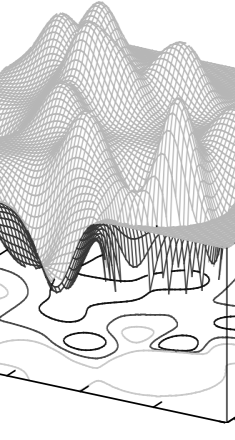
\includegraphics[height=7cm]{classPicture2-bw}
    }{\center

      \textbf{\fontsize{17}{20}\selectfont \course}

      ~

      %Lecture
      \topic\\

      \vspace{1cm}

      {\tiny~\emph{\keywords}~\\}

      \vspace{1cm}

      Marc Toussaint
      
      University of Stuttgart

      Summer 2019

      ~

    }
  }
}

\newcommand{\slide}[2]{
  \slidefont
  \incpage\begin{frame}
  \addcontentsline{toc}{section}{#1}
  \vfill
  {\headerfont #1} \vspace*{-2ex}
  \begin{itemize}\item[]~\\
    #2
  \end{itemize}
  \vfill
  \end{frame}
}

\newenvironment{slidecore}[1]{
  \slidefont\incpage
  \addcontentsline{toc}{section}{#1}
  \vfill
  {\headerfont #1} \vspace*{-2ex}
  \begin{itemize}\item[]~\\
}{
  \end{itemize}
  \vfill
}


\providecommand{\key}[1]{
  \addtocounter{mypage}{1}
% \immediate\write\keyfile{#1}
  \addtocontents{toc}{\hyperref[key:#1]{#1 (\arabic{mypage})}}
%  \phantomsection\label{key:#1}
%  \index{#1@{\hyperref[key:#1]{#1 (\arabic{mysec}:\arabic{mypage})}}|phantom}
  \addtocounter{mypage}{-1}
}

\providecommand{\course}{}

\providecommand{\subtopic}{}

\providecommand{\sublecture}[2]{
  \renewcommand{\subtopic}{#1}
  \slide{#1}{#2}
}

\providecommand{\story}[1]{
~

Motivation: {\tiny #1}\clearpage
}

\newenvironment{items}[1][9]{
\par\setlength{\unitlength}{1pt}\fontsize{#1}{#1}\linespread{1.2}\selectfont
\begin{list}{--}{\leftmargin4ex \rightmargin0ex \labelsep1ex \labelwidth2ex
\topsep0pt \parsep0ex \itemsep3pt}
}{
\end{list}
}

\providecommand{\slidesfoot}{
  \end{document}
}


  \slideshead
}

\providecommand{\exercises}{
  \newcommand{\exerciseshead}{
  \documentclass[10pt,fleqn]{article}
  \stdpackages

  \definecolor{bluecol}{rgb}{0,0,.5}
  \definecolor{greencol}{rgb}{0,.4,0}
  \definecolor{shadecolor}{gray}{0.9}
  \usepackage[
    %    pdftex%,
    %%    letterpaper,
    %    bookmarks,
    %    bookmarksnumbered,
    colorlinks,
    urlcolor=bluecol,
    citecolor=black,
    linkcolor=bluecol,
    %    pagecolor=bluecol,
    pdfborder={0 0 0},
    %pdfborderstyle={/S/U/W 1},
    %%    backref,     %link from bibliography back to sections
    %%    pagebackref, %link from bibliography back to pages
    %%    pdfstartview=FitH, %fitwidth instead of fit window
    pdfpagemode=UseNone, %UseOutlines, %bookmarks are displayed by acrobat
    pdftitle={\course},
    pdfauthor={Marc Toussaint},
    pdfkeywords={}
  ]{hyperref}
  \DeclareGraphicsExtensions{.pdf,.png,.jpg,.eps}

  \renewcommand{\r}{\varrho}
  \renewcommand{\l}{\lambda}
  \renewcommand{\L}{\Lambda}
  \renewcommand{\b}{\beta}
  \renewcommand{\d}{\delta}
  \renewcommand{\k}{\kappa}
  \renewcommand{\t}{\theta}
  \renewcommand{\O}{\Omega}
  \renewcommand{\o}{\omega}
  \renewcommand{\SS}{{\cal S}}
  \renewcommand{\=}{\!=\!}
  %\renewcommand{\boldsymbol}{}
  %\renewcommand{\Chapter}{\chapter}
  %\renewcommand{\Subsection}{\subsection}

  \renewcommand{\baselinestretch}{1.1}
  \geometry{a4paper,headsep=7mm,hdivide={15mm,*,15mm},vdivide={20mm,*,15mm}}

  \fancyhead[L]{\thetitle, \textit{Marc Toussaint}---\today}
  \fancyhead[R]{\thepage}
  \fancyhead[C]{}
  \fancyfoot{}
  \pagestyle{fancy}

  \parindent 0pt
  \parskip 0.5ex

  \newcommand{\codefont}{\helvetica{8}{1.2}{m}{n}}

  %auto-ignore
  \renewcommand{\a}{\alpha}
  \renewcommand{\b}{\beta}
  \renewcommand{\d}{\delta}
    \newcommand{\D}{\Delta}
    \newcommand{\e}{\epsilon}
    \newcommand{\g}{\gamma}
    \newcommand{\G}{\Gamma}
  \renewcommand{\l}{\lambda}
  \renewcommand{\L}{\Lambda}
    \newcommand{\m}{\mu}
    \newcommand{\n}{\nu}
    \newcommand{\N}{\nabla}
  \renewcommand{\k}{\kappa}
  \renewcommand{\o}{\omega}
  \renewcommand{\O}{\Omega}
    \newcommand{\p}{\phi}
    \newcommand{\ph}{\varphi}
  \renewcommand{\P}{\Phi}
  \renewcommand{\r}{\varrho}
    \newcommand{\s}{\sigma}
  \renewcommand{\S}{\Sigma}
  \renewcommand{\t}{\theta}
    \newcommand{\T}{\Theta}
  %\renewcommand{\v}{\vartheta}
    \newcommand{\x}{\xi}
    \newcommand{\X}{\Xi}
    \newcommand{\Y}{\Upsilon}
    \newcommand{\z}{\zeta}

  \renewcommand{\AA}{{\cal A}}
    \newcommand{\BB}{{\cal B}}
    \newcommand{\CC}{{\cal C}}
    \newcommand{\cc}{{\cal c}}
    \newcommand{\DD}{{\cal D}}
    \newcommand{\EE}{{\cal E}}
    \newcommand{\FF}{{\cal F}}
    \newcommand{\GG}{{\cal G}}
    \newcommand{\HH}{{\cal H}}
    \newcommand{\II}{{\cal I}}
    \newcommand{\KK}{{\cal K}}
    \newcommand{\LL}{{\cal L}}
    \newcommand{\MM}{{\cal M}}
    \newcommand{\NN}{{\cal N}}
    \newcommand{\oNN}{\overline\NN}
    \newcommand{\OO}{{\cal O}}
    \newcommand{\PP}{{\cal P}}
    \newcommand{\QQ}{{\cal Q}}
    \newcommand{\RR}{{\cal R}}
  \renewcommand{\SS}{{\cal S}}
    \newcommand{\TT}{{\cal T}}
    \newcommand{\uu}{{\cal u}}
    \newcommand{\UU}{{\cal U}}
    \newcommand{\VV}{{\cal V}}
    \newcommand{\XX}{{\cal X}}
    \newcommand{\xx}{\mathcal{x}}
    \newcommand{\YY}{{\cal Y}}
    \newcommand{\SOSO}{{\cal SO}}
    \newcommand{\GLGL}{{\cal GL}}

    \newcommand{\Ee}{{\rm E}}

  \newcommand{\NNN}{{\mathbb{N}}}
  \newcommand{\III}{{\mathbb{I}}}
  \newcommand{\ZZZ}{{\mathbb{Z}}}
  %\newcommand{\RRR}{{\mathrm{I\!R}}}
  \newcommand{\RRR}{{\mathbb{R}}}
  \newcommand{\SSS}{{\mathbb{S}}}
  \newcommand{\CCC}{{\mathbb{C}}}
  \newcommand{\DDD}{{\mathbb{D}}}
  \newcommand{\one}{{{\bf 1}}}
  \newcommand{\eee}{\text{e}}

  \newcommand{\NNNN}{{\overline{\cal N}}}

  \renewcommand{\[}{\Big[}
  \renewcommand{\]}{\Big]}
  \renewcommand{\(}{\Big(}
  \renewcommand{\)}{\Big)}
  \renewcommand{\|}{\,|\,}
  \renewcommand{\;}{\,;\,}
  \renewcommand{\=}{\!=\!}
    \newcommand{\<}{\left\langle}
  \renewcommand{\>}{\right\rangle}

  \newcommand{\na}[1][]{{\nabla_{\!\!#1}}}
  \newcommand{\he}[1][]{{\nabla_{\!\!#1}^2}}
  \newcommand{\Prob}{{\rm Prob}}
  \newcommand{\Dir}{{\rm Dir}}
  \newcommand{\Beta}{{\rm Beta}}
  \newcommand{\Bern}{{\rm Bern}}
  \newcommand{\Bin}{{\rm Bin}}
  \newcommand{\Mult}{{\rm Mult}}
  \newcommand{\Aut}{{\rm Aut}}
  \newcommand{\cor}{{\rm cor}}
  \newcommand{\corr}{{\rm corr}}
  \newcommand{\sd}{{\rm sd}}
  \newcommand{\tr}{{\rm tr}}
  \newcommand{\Tr}{{\rm Tr}}
  \newcommand{\rank}{{\rm rank}}
  \newcommand{\diag}{{\rm diag}}
  \newcommand{\dom}{{\rm dom}}
  \newcommand{\id}{{\rm id}}
  \newcommand{\Id}{{\rm\bf I}}
  \newcommand{\Gl}{{\rm Gl}}
  \renewcommand{\th}{\ensuremath{{}^\text{th}} }
  \newcommand{\lag}{\mathcal{L}}
  \newcommand{\inn}{\rfloor}
  \newcommand{\lie}{\pounds}
  \newcommand{\longto}{\longrightarrow}
  \newcommand{\speer}{\parbox{0.4ex}{\raisebox{0.8ex}{$\nearrow$}}}
  \renewcommand{\dag}{ {}^\dagger }
  \newcommand{\blbox}{\rule{1ex}{1ex}}
  \newcommand{\Ji}{J^\sharp}
  \newcommand{\h}{{}^\star}
  \newcommand{\w}{\wedge}
  \newcommand{\too}{\longrightarrow}
  \newcommand{\oot}{\longleftarrow}
  \newcommand{\To}{\Rightarrow}
  \newcommand{\oT}{\Leftarrow}
  \newcommand{\oTo}{\Leftrightarrow}
  \renewcommand{\iff}{~\Longleftrightarrow~}
  \newcommand{\Too}{\;\Longrightarrow\;}
  \newcommand{\oto}{\leftrightarrow}
  \newcommand{\ot}{\leftarrow}
  \newcommand{\ootoo}{\longleftrightarrow}
  \newcommand{\ow}{\stackrel{\circ}\wedge}
  \newcommand{\defeq}{\stackrel{\hspace{0.2ex}{}_\Delta}=}
%  \newcommand{\defeq}{{\overstack\Delta =}}
  \newcommand{\feed}{\nonumber \\}
  \newcommand{\comma}{~,\quad}
  \newcommand{\period}{~.\quad}
  \newcommand{\del}{\partial}
%  \newcommand{\quabla}{\Delta}
  \newcommand{\point}{$\bullet~~$}
  \newcommand{\doubletilde}{ ~ \raisebox{0.3ex}{$\widetilde {}$} \raisebox{0.6ex}{$\widetilde {}$} \!\! }
  \newcommand{\topcirc}{\parbox{0ex}{~\raisebox{2.5ex}{${}^\circ$}}}
  \newcommand{\topdot} {\parbox{0ex}{~\raisebox{2.5ex}{$\cdot$}}}
  \newcommand{\topddot} {\parbox{0ex}{~\raisebox{1.3ex}{$\ddot{~}$}}}
  \newcommand{\sym}{\topcirc}
  \newcommand{\tsum}{\textstyle\sum}
  \newcommand{\st}{\quad\text{s.t.}\quad}

  \newcommand{\half}{\ensuremath{\frac{1}{2}}}
  \newcommand{\third}{\ensuremath{\frac{1}{3}}}
  \newcommand{\fourth}{\ensuremath{\frac{1}{4}}}

  \newcommand{\ubar}{\underline}
  %\renewcommand{\vec}{\underline}
  \renewcommand{\vec}{\boldsymbol}
  %\renewcommand{\_}{\underset}
  %\renewcommand{\^}{\overset}
  %\renewcommand{\*}{{\rm\raisebox{-.6ex}{\text{*}}{}}}
  \renewcommand{\*}{\text{\footnotesize\raisebox{-.4ex}{*}{}}}

  \newcommand{\gto}{{\raisebox{.5ex}{${}_\rightarrow$}}}
  \newcommand{\gfrom}{{\raisebox{.5ex}{${}_\leftarrow$}}}
  \newcommand{\gnto}{{\raisebox{.5ex}{${}_\nrightarrow$}}}
  \newcommand{\gnfrom}{{\raisebox{.5ex}{${}_\nleftarrow$}}}

  %\newcommand{\RND}{{\SS}}
  %\newcommand{\IF}{\text{if }}
  %\newcommand{\AND}{\textsc{and }}
  %\newcommand{\OR}{\textsc{or }}
  %\newcommand{\XOR}{\textsc{xor }}
  %\newcommand{\NOT}{\textsc{not }}

  %\newcommand{\argmax}[1]{{\rm arg}\!\max_{#1}}
  %\newcommand{\argmin}[1]{{\rm arg}\!\min_{#1}}
  \DeclareMathOperator*{\argmax}{argmax}
  \DeclareMathOperator*{\argmin}{argmin}
  \DeclareMathOperator{\sign}{sign}
  \DeclareMathOperator{\acos}{acos}
  \DeclareMathOperator{\unifies}{unifies}
  \DeclareMathOperator{\Span}{span}
  \newcommand{\ortho}{\perp}
  %\newcommand{\argmax}[1]{\underset{~#1}{\text{argmax}}\;}
  %\newcommand{\argmin}[1]{\underset{~#1}{\text{argmin}}\;}
  \newcommand{\ee}[1]{\ensuremath{\cdot10^{#1}}}
  \newcommand{\sub}[1]{\ensuremath{_{\text{#1}}}}
  \newcommand{\up}[1]{\ensuremath{^{\text{#1}}}}
  \newcommand{\kld}[3][{}]{D_{#1}\big(#2\,\big|\!\big|\,#3\big)}
  %\newcommand{\kld}[2]{D\big(#1:#2\big)}
  \newcommand{\sprod}[2]{\big<#1\,,\,#2\big>}
  \newcommand{\End}{\text{End}}
  \newcommand{\txt}[1]{\quad\text{#1}\quad}
  \newcommand{\Over}[2]{\genfrac{}{}{0pt}{0}{#1}{#2}}
  %\newcommand{\mat}[1]{{\bf #1}}
  \newcommand{\arr}[2]{\hspace*{-.5ex}\begin{array}{#1}#2\end{array}\hspace*{-.5ex}}
  \newcommand{\mat}[3][.9]{
    \renewcommand{\arraystretch}{#1}{\scriptscriptstyle{\left(
      \hspace*{-1ex}\begin{array}{#2}#3\end{array}\hspace*{-1ex}
    \right)}}\renewcommand{\arraystretch}{1.2}
  }
  \newcommand{\Mat}[3][.9]{
    \renewcommand{\arraystretch}{#1}{\scriptscriptstyle{\left[
      \hspace*{-1ex}\begin{array}{#2}#3\end{array}\hspace*{-1ex}
    \right]}}\renewcommand{\arraystretch}{1.2}
  }
  \newcommand{\case}[2][ll]{\left\{\arr{#1}{#2}\right.}
  \newcommand{\seq}[1]{\textsf{\<#1\>}}
  \newcommand{\seqq}[1]{\textsf{#1}}
  \newcommand{\floor}[1]{\lfloor#1\rfloor}
  \newcommand{\Exp}[2][]{\text{E}_{#1}\{#2\}}
  \newcommand{\Var}[2][]{\text{Var}_{#1}\{#2\}}
  \newcommand{\cov}[2][]{\text{cov}_{#1}\{#2\}}

  %\newcommand{\Exp}[2]{\left\langle{#2}\right\rangle_{#1}}
  \newcommand{\ex}{\setminus}

  \providecommand{\href}[2]{{\color{blue}USE PDFLATEX!}}
  \providecommand{\url}[2]{\href{#1}{{\color{blue}#2}}}
%  \newcommand{\link}[1]{\href{{\protect #1}}{\texttt{\protect #1}}}
  \newcommand{\anchor}[2]{\begin{picture}(0,0)\put(#1){#2}\end{picture}}
  \newcommand{\pagebox}{\begin{picture}(0,0)\put(-3,-23){
    \textcolor[rgb]{.5,1,.5}{\framebox[\textwidth]{\rule[-\textheight]{0pt}{0pt}}}}
    \end{picture}}

  \newcommand{\hide}[1]{
    \begin{list}{}{\leftmargin0ex \rightmargin0ex \topsep0ex \parsep0ex}
       \helvetica{5}{1}{m}{n}
       \renewcommand{\section}{\par SECTION: }
       \renewcommand{\subsection}{\par SUBSECTION: }
       \item[$~~\blacktriangleright$]
       #1%$\blacktriangleleft~~$
       \message{^^JHIDE--Warning!^^J}
    \end{list}
  }
  %\newcommand{\hide}[1]{{\tt[hide:~}{\footnotesize\sf #1}{\tt]}\message{^^JHIDE--Warning!^^J}}
  \newcommand{\Hide}{\renewcommand{\hide}[1]{\message{^^JHIDE--Warning (hidden)!^^J}}}
  \newcommand{\HIDE}{\renewcommand{\hide}[1]{}}
  \newcommand{\fullhide}[1]{\message{^^JHIDE--Warning (hidden)!^^J}}
  \newcommand{\todo}[1]{{\tt[TODO: #1]}\message{^^JTODO--Warning: #1^^J}}
  \newcommand{\Todo}{\renewcommand{\todo}[1]{\message{^^JTODO--Warning (hidden)!^^J}}}
  %\renewcommand{\title}[1]{\renewcommand{\thetitle}{#1}}
  \newcommand{\myauthor}[1]{\author{#1}\newcommand{\theauthor}{#1}}%\@author}
  \newcommand{\mytitle}[1]{\title{#1}\newcommand{\thetitle}{#1}}%\@title}
  \newcommand{\header}{\begin{document}\mytitle\cleardefs}
  \newcommand{\contents}{{\tableofcontents}\renewcommand{\contents}{}}
  \newcommand{\footer}{\small\bibliography{marc,bibs}\end{document}}
  \newcommand{\widepaper}{\usepackage{geometry}\geometry{a4paper,hdivide={25mm,*,25mm},vdivide={25mm,*,25mm}}}
  \newcommand{\moviex}[2]{\movie[externalviewer]{#1}{#2}} %\pdflatex\usepackage{multimedia}
  \newcommand{\rbox}[1]{\fboxrule2mm\fcolorbox[rgb]{1,.85,.85}{1,.85,.85}{#1}}
  \newcommand{\mpage}[2]{{\begin{minipage}{#1\columnwidth}#2\end{minipage}}}
  \newcommand{\redbox}[2]{\fboxrule1mm\fcolorbox[rgb]{1,.7,.7}{1,.7,.7}{\begin{minipage}{#1\columnwidth}\center#2\end{minipage}}}
  \newcommand{\onecol}[2]{
    \begin{minipage}[c]{#1\columnwidth}#2\end{minipage}}
  \newcommand{\twocol}[5][0]{
    \begin{minipage}[c]{#2\columnwidth}#4\end{minipage}\hspace*{#1\columnwidth}%
    \begin{minipage}[c]{#3\columnwidth}#5\end{minipage}}
  \newcommand{\threecol}[7][0]{%
    \begin{minipage}[c]{#2\columnwidth}#5\end{minipage}\hspace*{#1\columnwidth}%
    \begin{minipage}[c]{#3\columnwidth}#6\end{minipage}\hspace*{#1\columnwidth}%
    \begin{minipage}[c]{#4\columnwidth}#7\end{minipage}}
  \newcommand{\threecoltext}[7][c]{
    \begin{minipage}[#1]{#2\textwidth}#5\end{minipage}%
    \begin{minipage}[#1]{#3\textwidth}#6\end{minipage}%
    \begin{minipage}[#1]{#4\textwidth}#7\end{minipage}}
  \newcommand{\threecoltop}[7][0]{%
   \begin{minipage}[t]{#2\columnwidth}#5\end{minipage}\hspace*{#1\columnwidth}%
   \begin{minipage}[t]{#3\columnwidth}#6\end{minipage}\hspace*{#1\columnwidth}%
   \begin{minipage}[t]{#4\columnwidth}#7\end{minipage}}
  \newcommand{\fourcol}[9][0]{%
   \begin{minipage}[c]{#2\columnwidth}#6\end{minipage}\hspace*{#1\columnwidth}%
   \begin{minipage}[c]{#3\columnwidth}#7\end{minipage}\hspace*{#1\columnwidth}%
   \begin{minipage}[c]{#4\columnwidth}#8\end{minipage}\hspace*{#1\columnwidth}%
   \begin{minipage}[c]{#5\columnwidth}#9\end{minipage}}
  \newcommand{\helvetica}[4]{\setlength{\unitlength}{1pt}\fontsize{#1}{#1}\linespread{#2}\usefont{OT1}{phv}{#3}{#4}}
  \newcommand{\helve}[1]{\helvetica{#1}{1.5}{m}{n}}
  \newcommand{\german}{\usepackage[german]{babel}\usepackage[utf8]{inputenc}}

\newcommand{\norm}[1]{|\!|#1|\!|}
\newcommand{\expr}[1]{[\hspace{-.2ex}[#1]\hspace{-.2ex}]}

\newcommand{\Jwi}{J^\sharp_W}
\newcommand{\THi}{T^\sharp_H}
\newcommand{\Jci}{J^\natural_C}
\newcommand{\hJi}{{\bar J}^\sharp}
\renewcommand{\|}{\,|\,}
\renewcommand{\=}{\!=\!}
\newcommand{\myminus}{{\hspace*{-.0pt}\text{\rm -}\hspace*{-.5pt}}}
\newcommand{\myplus}{{\hspace*{-.0pt}\text{\rm +}\hspace*{-.5pt}}}
\newcommand{\1}{{\myminus1}}
\newcommand{\2}{{\myminus2}}
\newcommand{\3}{{\myminus3}}
\newcommand{\mT}{{\text{\rm -}\hspace*{-1pt}\top}}
\newcommand{\po}{{\myplus1}}
\newcommand{\pt}{{\myplus2}}
%\renewcommand{\-}{\myminus}
%\newcommand{\+}{\myplus}
\renewcommand{\T}{{\!\top\!}}
\newcommand{\xT}{{\underline x}}
\newcommand{\uT}{{\underline u}}
\newcommand{\zT}{{\underline z}}
\newcommand{\Sum}{\textstyle\sum}
\newcommand{\Int}{\textstyle\int}
\newcommand{\Prod}{\textstyle\prod}


\newenvironment{centy}{
\vspace{15mm}
\large
\hspace*{5mm}
\begin{minipage}{8cm}\it\color{blue}
}{
\end{minipage}
}

\newcommand{\old}{{\text{old}}}
\newcommand{\new}{{\text{new}}}
\newcommand{\MAP}{{\text{MAP}}}
\newcommand{\ML}{{\text{ML}}}

\newcommand{\redArrow}{\quad\anchor{0,-1}{\includegraphics[scale=.5]{figs/redArrow}}}
\newcommand{\pub}[1]{{\color{green}\helvetica{8}{1.3}{m}{n}#1\\}}
\DeclareMathOperator{\opKL}{KL}
\newcommand{\KL}[2]{\opKL\big(#1\,\big|\!\big|\,#2\big)} %\left(#1 |\!| #2\right)}

\renewcommand{\show}[2][.8]{\centerline{\includegraphics[width=#1\columnwidth]{#2}}}
\newcommand{\showh}[2][.8]{\includegraphics[width=#1\columnwidth]{#2}}
\newcommand{\shows}[2][.8]{\centerline{\includegraphics[scale=#1]{#2}}}
\newcommand{\showhs}[2][.8]{\includegraphics[scale=#1]{#2}}
\newcommand{\mov}[2]{\movie[externalviewer]{{\color{blue}\small #1}}{movies/#2}}
\newcommand{\movex}[2]{\movie[externalviewer]{#1}{#2}} %\pdflatex\usepackage{multimedia}
%\newcommand{\movgb}[1]{\hfill\movie[externalviewer]{\small[movie]}{/home/mtoussai/movies/10-goalDirectedBehavior/#1}}
\newcommand{\movh}[3][loop]{
\movie[#1]{\showh[#2]{movies/#3.png}}{movies/#3.avi}%
\movie[externalviewer]{$\circ$}{movies/#3.avi}
}
\newcommand{\movc}[3][loop]{\centerline{\movh[#1]{#2}{#3}}}
\newcommand{\cen}[1]{\centerline{#1}}

\newcommand{\citing}[1]{
{\color{citcol}\tiny#1\par}
}

\newcommand{\cit}[3]{
\par\smallskip
{\color{greencol}\tiny #1: \emph{#2}. #3 \par}
}

\newcommand{\citurl}[4]{
\par\smallskip
{\color{greencol}\tiny #1: \protect{\href{#4}{\color{blue}{#2.}}} #3 \par}
}

\newcommand{\cito}[3]{
\par\smallskip
{\color{bluecol}\tiny #1: \emph{#2}. #3 \par}
}

\newcommand{\redoMacrosInProof}{
  \renewcommand{\d}{\delta}
%  \renewcommand{\|}{\,|\,}
  \renewcommand{\=}{\!=\!}
}

%% \makeatletter
%% \newenvironment{code}{%
%%   \begin{lrbox}{\@tempboxa}\begin{minipage}{1\columnwidth}\codefont
%% }{
%%   \end{minipage}\end{lrbox}%
%%   \colorbox[rgb]{.95,.95,.95}{\usebox{\@tempboxa}}
%% }\makeatother

\newenvironment{code}{%
\codefont
\begin{shaded}
}{
\end{shaded}
}

%\newcommand{\refeq}[1]{(\ref{#1})}

\usepackage{algorithm}
\usepackage{algpseudocode}
\algrenewcommand{\algorithmicrequire}{\textbf{Input:~~}}
\algrenewcommand{\algorithmicensure}{\textbf{Output:}}
\algrenewcommand{\algorithmiccomment}[1]{\qquad\hfill~\hspace*{-5ex}\textit{// #1}}
\algrenewcommand{\alglinenumber}[1]{\helvetica{6}{1.3}{m}{n}#1:}

\newenvironment{algo}[1][8]{
\quad\begin{minipage}{.8\columnwidth}\helvetica{#1}{1.3}{m}{n}
\medskip\hrule\medskip
\begin{algorithmic}[1]
}{
\end{algorithmic}
\medskip\hrule\medskip
\end{minipage}
}

\usepackage{etoolbox}

%%%%%%%%%%%%%%%%%%%%%%%%%%%%%%%%%%%%%%%%%%%%%%%%%%%%%%%%%%%%%%%%%%%%%%%%%%%%%%%%

\usepackage{multirow}
\usepackage{colortbl}
%\setlength{\jot}{0pt}
%\setlength{\mathindent}{1ex}
\usepackage{empheq}

%%%%%%%%%%%%%%%%%%%%%%%%%%%%%%%%%%%%%%%%%%%%%%%%%%%%%%%%%%%%%%%%%%%%%%%%%%%%%%%

\newcommand{\mypause}{\pause}
%\newcommand{\dom}{{\text{dom}}}
\newcommand{\defi}[1]{\textbf{#1}}
\newcommand{\red}[1]{\emph{\color{red}#1}}
%\newcommand{\ul}{\underline}
\newcommand{\pos}{{\textsf{pos}}}
\newcommand{\eff}{{\textsf{eff}}}
\newcommand{\rot}{{\textsf{rot}}}
\newcommand{\veC}{{\textsf{vec}}}
\newcommand{\quat}{{\textsf{quat}}}
\newcommand{\col}{{\textsf{col}}}
\newcommand{\de}[2]{\frac{\partial #1}{\partial #2}}
\newcommand{\target}{{\text{target}}}
\newcommand{\near}{{\text{near}}}
\newcommand{\qfree}{Q_{\text{free}}}
\renewcommand{\vec}{\boldsymbol}
\newcommand{\lft}{\text{left}}
\newcommand{\rgh}{\text{right}}
\DeclareMathOperator{\real}{real}
\newcommand{\prev}{{\text{prev}}}
\newcommand{\TR}[2]{T_{{#1}\shortrightarrow{#2}}}
\newcommand{\RO}[2]{R_{{#1}\shortrightarrow{#2}}}
\newcommand{\liter}{\helvetica{8}{1.1}{m}{n}\parskip 1ex}
\newcommand{\Fc}{\color{green}F}
\newcommand{\muc}{\color{blue}\mu}
\newcommand{\Astar}{A$^*$}

%for optimization course:
\newcommand{\adec}{\r_\a^-}
\newcommand{\ainc}{\r_\a^+}
\newcommand{\ldec}{\r_\l^-}
\newcommand{\linc}{\r_\l^+}
\newcommand{\minc}{\r_\m^+}
\newcommand{\mdec}{\r_\m^-}
\newcommand{\lsstop}{\r_{\text{ls}}}


\definecolor{boxcol}{rgb}{.85,.9,.92}
\newcommand{\eqbox}[1]{\centerline{\fboxrule0mm\fcolorbox{boxcol}{boxcol}{#1}}}
\newcommand{\movgb}[1]{\hfill\movie[externalviewer]{\small[movie]}{/home/mtoussai/movies/10-goalDirectedBehavior/#1}}
\newcommand{\demo}[1]{{{\color{blue}[\small #1]}}}

\graphicspath{{../pics-robotics/}{../pics-ML/}{../pics-all/}{../pics-all2/}{../pics-Optim/}}
\DeclareGraphicsExtensions{.pdf,.png,.jpg}

%\usepackage{pdfpages}
%\setbeamercolor{background canvas}{bg=}

\newcommand{\SUM}{\texttt{sum}}
\usepackage{float}

%% prevent pagebreaks before environment
\makeatletter
\newcommand{\NewParNoBreak}[1][\parskip]{\par\vspace*{-\parskip}\vspace*{#1}\nobreak\@afterheading}
\makeatother

%\newcommand{\idx}[2]{\label{IKgn}}

%%%%%%%%%%%%%%%%%%%%%%%%%%%%%%%%%%%%%%%%%%%%%%%%%%%%%%%%%%%%%%%%%%%%%%%%%%%%%%%%



%% \newwrite\tempfile
%% \immediate\openout\tempfile=z.keys.tex

%% \renewcommand{\key}[1]{
%% %%   \addtocounter{mypage}{1}
%% \makeatletter
%% \immediate\write\tempfile{\symbol{`\\}}
%% \makeatother
%%   \immediate\write\tempfile{hyperref[key:#1]{#1(\arabic{mypage})}}
%% %%  % \phantomsection\label{key:#1}
%% %%   %\index{#1@{\hyperref[key:#1]{#1 (\arabic{mysec}:\arabic{mypage})}}|phantom}
%% %%   \addtocounter{mypage}{-1}
%% }


  \DefineShortVerb{\@}

  \newcounter{solutions}
  \setcounter{solutions}{1}
  \newenvironment{solution}{
    \small
    \begin{shaded}
  }{
    \end{shaded}
  }
  
  \renewcommand{\hat}{\widehat}
  \newcommand{\bbg}{{\bar{\bar g}}}
  \graphicspath{{pics/}{../shared/pics/}}

  \renewcommand{\labelenumi}{{\alph{enumi})}}

  %%%%%%%%%%%%%%%%%%%%%%%%%%%%%%%%%%%%%%%%%%%%%%%%%%%%%%%%%%%%%%%%%%%%%%%%%%%%%%%%


  \mytitle{\course\\Exercise \exnum}
  \myauthor{Marc Toussaint\\ TAs: Janik Hager, Philipp Kratzer\\\small\addressUSTT}
  
  
  \begin{document}
  \onecolumn
  \maketitle
}

\newcommand{\exsection}[1]{\section{#1}}

\newcommand{\exerfoot}{
  \end{document}
}

\newenvironment{items}[1][9]{
  \par\setlength{\unitlength}{1pt}\fontsize{#1}{#1}\linespread{1.2}\selectfont
  \begin{list}{--}{\leftmargin4ex \rightmargin0ex \labelsep1ex \labelwidth2ex
      \topsep0pt \parsep0ex \itemsep3pt}
}{
  \end{list}
}

  \exerciseshead
}

\providecommand{\script}{
  \newcommand{\scripthead}{
  \documentclass[9pt,twoside]{article}
  \stdpackages

  \usepackage{palatino}
  \usepackage[envcountsect]{beamerarticle}
  \usepackage{makeidx}
  \makeindex

  \definecolor{bluecol}{rgb}{0,0,.5}
  \definecolor{greencol}{rgb}{0,.4,0}
  \definecolor{shadecolor}{gray}{0.9}
  \usepackage[
    %    pdftex%,
    %%    letterpaper,
    %bookmarks,
    bookmarksnumbered,
    colorlinks,
    urlcolor=bluecol,
    citecolor=black,
    linkcolor=bluecol,
    %    pagecolor=bluecol,
    pdfborder={0 0 0},
    %pdfborderstyle={/S/U/W 1},
    %%    backref,     %link from bibliography back to sections
    %%    pagebackref, %link from bibliography back to pages
    %%    pdfstartview=FitH, %fitwidth instead of fit window
    pdfpagemode=UseOutlines, %bookmarks are displayed by acrobat
    pdftitle={\course},
    pdfauthor={Marc Toussaint},
    pdfkeywords={}
  ]{hyperref}
  \DeclareGraphicsExtensions{.pdf,.png,.jpg,.eps}

  \usepackage{multimedia}
  %\setbeamercolor{background canvas}{bg=}

  \renewcommand{\r}{\varrho}
  \renewcommand{\l}{\lambda}
  \renewcommand{\L}{\Lambda}
  \renewcommand{\b}{\beta}
  \renewcommand{\d}{\delta}
  \renewcommand{\k}{\kappa}
  \renewcommand{\t}{\theta}
  \renewcommand{\O}{\Omega}
  \renewcommand{\o}{\omega}
  \renewcommand{\SS}{{\cal S}}
  \renewcommand{\=}{\!=\!}
  %\renewcommand{\boldsymbol}{}
  %\renewcommand{\Chapter}{\chapter}
  %\renewcommand{\Subsection}{\subsection}

  \renewcommand{\baselinestretch}{1.0}
  \geometry{a5paper,headsep=6mm,hdivide={10mm,*,10mm},vdivide={13mm,*,7mm}}

  \fancyhead[OL,ER]{\course, \textit{Marc Toussaint}}
  \fancyhead[OR,EL]{\thepage}
  \fancyhead[C]{}
  \fancyfoot{}
  \pagestyle{fancy}

%  \setcounter{tocdepth}{3}
  \setcounter{tocdepth}{2}

   \columnsep 6ex
  %  \renewcommand{\familydefault}{\sfdefault}
  \newcommand{\headerfont}{\large}%helvetica{12}{1}{b}{n}}
  \newcommand{\slidefont} {}%\helvetica{9}{1.3}{m}{n}}
  \newcommand{\storyfont} {}
  %  \renewcommand{\small}   {\helvetica{8}{1.2}{m}{n}}
  \renewcommand{\tiny}    {\footnotesize}%helvetica{7}{1.1}{m}{n}}
  \newcommand{\codefont}{\fontsize{6}{6}\selectfont}%helvetica{8}{1.2}{m}{n}}

  %auto-ignore
  \renewcommand{\a}{\alpha}
  \renewcommand{\b}{\beta}
  \renewcommand{\d}{\delta}
    \newcommand{\D}{\Delta}
    \newcommand{\e}{\epsilon}
    \newcommand{\g}{\gamma}
    \newcommand{\G}{\Gamma}
  \renewcommand{\l}{\lambda}
  \renewcommand{\L}{\Lambda}
    \newcommand{\m}{\mu}
    \newcommand{\n}{\nu}
    \newcommand{\N}{\nabla}
  \renewcommand{\k}{\kappa}
  \renewcommand{\o}{\omega}
  \renewcommand{\O}{\Omega}
    \newcommand{\p}{\phi}
    \newcommand{\ph}{\varphi}
  \renewcommand{\P}{\Phi}
  \renewcommand{\r}{\varrho}
    \newcommand{\s}{\sigma}
  \renewcommand{\S}{\Sigma}
  \renewcommand{\t}{\theta}
    \newcommand{\T}{\Theta}
  %\renewcommand{\v}{\vartheta}
    \newcommand{\x}{\xi}
    \newcommand{\X}{\Xi}
    \newcommand{\Y}{\Upsilon}
    \newcommand{\z}{\zeta}

  \renewcommand{\AA}{{\cal A}}
    \newcommand{\BB}{{\cal B}}
    \newcommand{\CC}{{\cal C}}
    \newcommand{\cc}{{\cal c}}
    \newcommand{\DD}{{\cal D}}
    \newcommand{\EE}{{\cal E}}
    \newcommand{\FF}{{\cal F}}
    \newcommand{\GG}{{\cal G}}
    \newcommand{\HH}{{\cal H}}
    \newcommand{\II}{{\cal I}}
    \newcommand{\KK}{{\cal K}}
    \newcommand{\LL}{{\cal L}}
    \newcommand{\MM}{{\cal M}}
    \newcommand{\NN}{{\cal N}}
    \newcommand{\oNN}{\overline\NN}
    \newcommand{\OO}{{\cal O}}
    \newcommand{\PP}{{\cal P}}
    \newcommand{\QQ}{{\cal Q}}
    \newcommand{\RR}{{\cal R}}
  \renewcommand{\SS}{{\cal S}}
    \newcommand{\TT}{{\cal T}}
    \newcommand{\uu}{{\cal u}}
    \newcommand{\UU}{{\cal U}}
    \newcommand{\VV}{{\cal V}}
    \newcommand{\XX}{{\cal X}}
    \newcommand{\xx}{\mathcal{x}}
    \newcommand{\YY}{{\cal Y}}
    \newcommand{\SOSO}{{\cal SO}}
    \newcommand{\GLGL}{{\cal GL}}

    \newcommand{\Ee}{{\rm E}}

  \newcommand{\NNN}{{\mathbb{N}}}
  \newcommand{\III}{{\mathbb{I}}}
  \newcommand{\ZZZ}{{\mathbb{Z}}}
  %\newcommand{\RRR}{{\mathrm{I\!R}}}
  \newcommand{\RRR}{{\mathbb{R}}}
  \newcommand{\SSS}{{\mathbb{S}}}
  \newcommand{\CCC}{{\mathbb{C}}}
  \newcommand{\DDD}{{\mathbb{D}}}
  \newcommand{\one}{{{\bf 1}}}
  \newcommand{\eee}{\text{e}}

  \newcommand{\NNNN}{{\overline{\cal N}}}

  \renewcommand{\[}{\Big[}
  \renewcommand{\]}{\Big]}
  \renewcommand{\(}{\Big(}
  \renewcommand{\)}{\Big)}
  \renewcommand{\|}{\,|\,}
  \renewcommand{\;}{\,;\,}
  \renewcommand{\=}{\!=\!}
    \newcommand{\<}{\left\langle}
  \renewcommand{\>}{\right\rangle}

  \newcommand{\na}[1][]{{\nabla_{\!\!#1}}}
  \newcommand{\he}[1][]{{\nabla_{\!\!#1}^2}}
  \newcommand{\Prob}{{\rm Prob}}
  \newcommand{\Dir}{{\rm Dir}}
  \newcommand{\Beta}{{\rm Beta}}
  \newcommand{\Bern}{{\rm Bern}}
  \newcommand{\Bin}{{\rm Bin}}
  \newcommand{\Mult}{{\rm Mult}}
  \newcommand{\Aut}{{\rm Aut}}
  \newcommand{\cor}{{\rm cor}}
  \newcommand{\corr}{{\rm corr}}
  \newcommand{\sd}{{\rm sd}}
  \newcommand{\tr}{{\rm tr}}
  \newcommand{\Tr}{{\rm Tr}}
  \newcommand{\rank}{{\rm rank}}
  \newcommand{\diag}{{\rm diag}}
  \newcommand{\dom}{{\rm dom}}
  \newcommand{\id}{{\rm id}}
  \newcommand{\Id}{{\rm\bf I}}
  \newcommand{\Gl}{{\rm Gl}}
  \renewcommand{\th}{\ensuremath{{}^\text{th}} }
  \newcommand{\lag}{\mathcal{L}}
  \newcommand{\inn}{\rfloor}
  \newcommand{\lie}{\pounds}
  \newcommand{\longto}{\longrightarrow}
  \newcommand{\speer}{\parbox{0.4ex}{\raisebox{0.8ex}{$\nearrow$}}}
  \renewcommand{\dag}{ {}^\dagger }
  \newcommand{\blbox}{\rule{1ex}{1ex}}
  \newcommand{\Ji}{J^\sharp}
  \newcommand{\h}{{}^\star}
  \newcommand{\w}{\wedge}
  \newcommand{\too}{\longrightarrow}
  \newcommand{\oot}{\longleftarrow}
  \newcommand{\To}{\Rightarrow}
  \newcommand{\oT}{\Leftarrow}
  \newcommand{\oTo}{\Leftrightarrow}
  \renewcommand{\iff}{~\Longleftrightarrow~}
  \newcommand{\Too}{\;\Longrightarrow\;}
  \newcommand{\oto}{\leftrightarrow}
  \newcommand{\ot}{\leftarrow}
  \newcommand{\ootoo}{\longleftrightarrow}
  \newcommand{\ow}{\stackrel{\circ}\wedge}
  \newcommand{\defeq}{\stackrel{\hspace{0.2ex}{}_\Delta}=}
%  \newcommand{\defeq}{{\overstack\Delta =}}
  \newcommand{\feed}{\nonumber \\}
  \newcommand{\comma}{~,\quad}
  \newcommand{\period}{~.\quad}
  \newcommand{\del}{\partial}
%  \newcommand{\quabla}{\Delta}
  \newcommand{\point}{$\bullet~~$}
  \newcommand{\doubletilde}{ ~ \raisebox{0.3ex}{$\widetilde {}$} \raisebox{0.6ex}{$\widetilde {}$} \!\! }
  \newcommand{\topcirc}{\parbox{0ex}{~\raisebox{2.5ex}{${}^\circ$}}}
  \newcommand{\topdot} {\parbox{0ex}{~\raisebox{2.5ex}{$\cdot$}}}
  \newcommand{\topddot} {\parbox{0ex}{~\raisebox{1.3ex}{$\ddot{~}$}}}
  \newcommand{\sym}{\topcirc}
  \newcommand{\tsum}{\textstyle\sum}
  \newcommand{\st}{\quad\text{s.t.}\quad}

  \newcommand{\half}{\ensuremath{\frac{1}{2}}}
  \newcommand{\third}{\ensuremath{\frac{1}{3}}}
  \newcommand{\fourth}{\ensuremath{\frac{1}{4}}}

  \newcommand{\ubar}{\underline}
  %\renewcommand{\vec}{\underline}
  \renewcommand{\vec}{\boldsymbol}
  %\renewcommand{\_}{\underset}
  %\renewcommand{\^}{\overset}
  %\renewcommand{\*}{{\rm\raisebox{-.6ex}{\text{*}}{}}}
  \renewcommand{\*}{\text{\footnotesize\raisebox{-.4ex}{*}{}}}

  \newcommand{\gto}{{\raisebox{.5ex}{${}_\rightarrow$}}}
  \newcommand{\gfrom}{{\raisebox{.5ex}{${}_\leftarrow$}}}
  \newcommand{\gnto}{{\raisebox{.5ex}{${}_\nrightarrow$}}}
  \newcommand{\gnfrom}{{\raisebox{.5ex}{${}_\nleftarrow$}}}

  %\newcommand{\RND}{{\SS}}
  %\newcommand{\IF}{\text{if }}
  %\newcommand{\AND}{\textsc{and }}
  %\newcommand{\OR}{\textsc{or }}
  %\newcommand{\XOR}{\textsc{xor }}
  %\newcommand{\NOT}{\textsc{not }}

  %\newcommand{\argmax}[1]{{\rm arg}\!\max_{#1}}
  %\newcommand{\argmin}[1]{{\rm arg}\!\min_{#1}}
  \DeclareMathOperator*{\argmax}{argmax}
  \DeclareMathOperator*{\argmin}{argmin}
  \DeclareMathOperator{\sign}{sign}
  \DeclareMathOperator{\acos}{acos}
  \DeclareMathOperator{\unifies}{unifies}
  \DeclareMathOperator{\Span}{span}
  \newcommand{\ortho}{\perp}
  %\newcommand{\argmax}[1]{\underset{~#1}{\text{argmax}}\;}
  %\newcommand{\argmin}[1]{\underset{~#1}{\text{argmin}}\;}
  \newcommand{\ee}[1]{\ensuremath{\cdot10^{#1}}}
  \newcommand{\sub}[1]{\ensuremath{_{\text{#1}}}}
  \newcommand{\up}[1]{\ensuremath{^{\text{#1}}}}
  \newcommand{\kld}[3][{}]{D_{#1}\big(#2\,\big|\!\big|\,#3\big)}
  %\newcommand{\kld}[2]{D\big(#1:#2\big)}
  \newcommand{\sprod}[2]{\big<#1\,,\,#2\big>}
  \newcommand{\End}{\text{End}}
  \newcommand{\txt}[1]{\quad\text{#1}\quad}
  \newcommand{\Over}[2]{\genfrac{}{}{0pt}{0}{#1}{#2}}
  %\newcommand{\mat}[1]{{\bf #1}}
  \newcommand{\arr}[2]{\hspace*{-.5ex}\begin{array}{#1}#2\end{array}\hspace*{-.5ex}}
  \newcommand{\mat}[3][.9]{
    \renewcommand{\arraystretch}{#1}{\scriptscriptstyle{\left(
      \hspace*{-1ex}\begin{array}{#2}#3\end{array}\hspace*{-1ex}
    \right)}}\renewcommand{\arraystretch}{1.2}
  }
  \newcommand{\Mat}[3][.9]{
    \renewcommand{\arraystretch}{#1}{\scriptscriptstyle{\left[
      \hspace*{-1ex}\begin{array}{#2}#3\end{array}\hspace*{-1ex}
    \right]}}\renewcommand{\arraystretch}{1.2}
  }
  \newcommand{\case}[2][ll]{\left\{\arr{#1}{#2}\right.}
  \newcommand{\seq}[1]{\textsf{\<#1\>}}
  \newcommand{\seqq}[1]{\textsf{#1}}
  \newcommand{\floor}[1]{\lfloor#1\rfloor}
  \newcommand{\Exp}[2][]{\text{E}_{#1}\{#2\}}
  \newcommand{\Var}[2][]{\text{Var}_{#1}\{#2\}}
  \newcommand{\cov}[2][]{\text{cov}_{#1}\{#2\}}

  %\newcommand{\Exp}[2]{\left\langle{#2}\right\rangle_{#1}}
  \newcommand{\ex}{\setminus}

  \providecommand{\href}[2]{{\color{blue}USE PDFLATEX!}}
  \providecommand{\url}[2]{\href{#1}{{\color{blue}#2}}}
%  \newcommand{\link}[1]{\href{{\protect #1}}{\texttt{\protect #1}}}
  \newcommand{\anchor}[2]{\begin{picture}(0,0)\put(#1){#2}\end{picture}}
  \newcommand{\pagebox}{\begin{picture}(0,0)\put(-3,-23){
    \textcolor[rgb]{.5,1,.5}{\framebox[\textwidth]{\rule[-\textheight]{0pt}{0pt}}}}
    \end{picture}}

  \newcommand{\hide}[1]{
    \begin{list}{}{\leftmargin0ex \rightmargin0ex \topsep0ex \parsep0ex}
       \helvetica{5}{1}{m}{n}
       \renewcommand{\section}{\par SECTION: }
       \renewcommand{\subsection}{\par SUBSECTION: }
       \item[$~~\blacktriangleright$]
       #1%$\blacktriangleleft~~$
       \message{^^JHIDE--Warning!^^J}
    \end{list}
  }
  %\newcommand{\hide}[1]{{\tt[hide:~}{\footnotesize\sf #1}{\tt]}\message{^^JHIDE--Warning!^^J}}
  \newcommand{\Hide}{\renewcommand{\hide}[1]{\message{^^JHIDE--Warning (hidden)!^^J}}}
  \newcommand{\HIDE}{\renewcommand{\hide}[1]{}}
  \newcommand{\fullhide}[1]{\message{^^JHIDE--Warning (hidden)!^^J}}
  \newcommand{\todo}[1]{{\tt[TODO: #1]}\message{^^JTODO--Warning: #1^^J}}
  \newcommand{\Todo}{\renewcommand{\todo}[1]{\message{^^JTODO--Warning (hidden)!^^J}}}
  %\renewcommand{\title}[1]{\renewcommand{\thetitle}{#1}}
  \newcommand{\myauthor}[1]{\author{#1}\newcommand{\theauthor}{#1}}%\@author}
  \newcommand{\mytitle}[1]{\title{#1}\newcommand{\thetitle}{#1}}%\@title}
  \newcommand{\header}{\begin{document}\mytitle\cleardefs}
  \newcommand{\contents}{{\tableofcontents}\renewcommand{\contents}{}}
  \newcommand{\footer}{\small\bibliography{marc,bibs}\end{document}}
  \newcommand{\widepaper}{\usepackage{geometry}\geometry{a4paper,hdivide={25mm,*,25mm},vdivide={25mm,*,25mm}}}
  \newcommand{\moviex}[2]{\movie[externalviewer]{#1}{#2}} %\pdflatex\usepackage{multimedia}
  \newcommand{\rbox}[1]{\fboxrule2mm\fcolorbox[rgb]{1,.85,.85}{1,.85,.85}{#1}}
  \newcommand{\mpage}[2]{{\begin{minipage}{#1\columnwidth}#2\end{minipage}}}
  \newcommand{\redbox}[2]{\fboxrule1mm\fcolorbox[rgb]{1,.7,.7}{1,.7,.7}{\begin{minipage}{#1\columnwidth}\center#2\end{minipage}}}
  \newcommand{\onecol}[2]{
    \begin{minipage}[c]{#1\columnwidth}#2\end{minipage}}
  \newcommand{\twocol}[5][0]{
    \begin{minipage}[c]{#2\columnwidth}#4\end{minipage}\hspace*{#1\columnwidth}%
    \begin{minipage}[c]{#3\columnwidth}#5\end{minipage}}
  \newcommand{\threecol}[7][0]{%
    \begin{minipage}[c]{#2\columnwidth}#5\end{minipage}\hspace*{#1\columnwidth}%
    \begin{minipage}[c]{#3\columnwidth}#6\end{minipage}\hspace*{#1\columnwidth}%
    \begin{minipage}[c]{#4\columnwidth}#7\end{minipage}}
  \newcommand{\threecoltext}[7][c]{
    \begin{minipage}[#1]{#2\textwidth}#5\end{minipage}%
    \begin{minipage}[#1]{#3\textwidth}#6\end{minipage}%
    \begin{minipage}[#1]{#4\textwidth}#7\end{minipage}}
  \newcommand{\threecoltop}[7][0]{%
   \begin{minipage}[t]{#2\columnwidth}#5\end{minipage}\hspace*{#1\columnwidth}%
   \begin{minipage}[t]{#3\columnwidth}#6\end{minipage}\hspace*{#1\columnwidth}%
   \begin{minipage}[t]{#4\columnwidth}#7\end{minipage}}
  \newcommand{\fourcol}[9][0]{%
   \begin{minipage}[c]{#2\columnwidth}#6\end{minipage}\hspace*{#1\columnwidth}%
   \begin{minipage}[c]{#3\columnwidth}#7\end{minipage}\hspace*{#1\columnwidth}%
   \begin{minipage}[c]{#4\columnwidth}#8\end{minipage}\hspace*{#1\columnwidth}%
   \begin{minipage}[c]{#5\columnwidth}#9\end{minipage}}
  \newcommand{\helvetica}[4]{\setlength{\unitlength}{1pt}\fontsize{#1}{#1}\linespread{#2}\usefont{OT1}{phv}{#3}{#4}}
  \newcommand{\helve}[1]{\helvetica{#1}{1.5}{m}{n}}
  \newcommand{\german}{\usepackage[german]{babel}\usepackage[utf8]{inputenc}}

\newcommand{\norm}[1]{|\!|#1|\!|}
\newcommand{\expr}[1]{[\hspace{-.2ex}[#1]\hspace{-.2ex}]}

\newcommand{\Jwi}{J^\sharp_W}
\newcommand{\THi}{T^\sharp_H}
\newcommand{\Jci}{J^\natural_C}
\newcommand{\hJi}{{\bar J}^\sharp}
\renewcommand{\|}{\,|\,}
\renewcommand{\=}{\!=\!}
\newcommand{\myminus}{{\hspace*{-.0pt}\text{\rm -}\hspace*{-.5pt}}}
\newcommand{\myplus}{{\hspace*{-.0pt}\text{\rm +}\hspace*{-.5pt}}}
\newcommand{\1}{{\myminus1}}
\newcommand{\2}{{\myminus2}}
\newcommand{\3}{{\myminus3}}
\newcommand{\mT}{{\text{\rm -}\hspace*{-1pt}\top}}
\newcommand{\po}{{\myplus1}}
\newcommand{\pt}{{\myplus2}}
%\renewcommand{\-}{\myminus}
%\newcommand{\+}{\myplus}
\renewcommand{\T}{{\!\top\!}}
\newcommand{\xT}{{\underline x}}
\newcommand{\uT}{{\underline u}}
\newcommand{\zT}{{\underline z}}
\newcommand{\Sum}{\textstyle\sum}
\newcommand{\Int}{\textstyle\int}
\newcommand{\Prod}{\textstyle\prod}


\newenvironment{centy}{
\vspace{15mm}
\large
\hspace*{5mm}
\begin{minipage}{8cm}\it\color{blue}
}{
\end{minipage}
}

\newcommand{\old}{{\text{old}}}
\newcommand{\new}{{\text{new}}}
\newcommand{\MAP}{{\text{MAP}}}
\newcommand{\ML}{{\text{ML}}}

\newcommand{\redArrow}{\quad\anchor{0,-1}{\includegraphics[scale=.5]{figs/redArrow}}}
\newcommand{\pub}[1]{{\color{green}\helvetica{8}{1.3}{m}{n}#1\\}}
\DeclareMathOperator{\opKL}{KL}
\newcommand{\KL}[2]{\opKL\big(#1\,\big|\!\big|\,#2\big)} %\left(#1 |\!| #2\right)}

\renewcommand{\show}[2][.8]{\centerline{\includegraphics[width=#1\columnwidth]{#2}}}
\newcommand{\showh}[2][.8]{\includegraphics[width=#1\columnwidth]{#2}}
\newcommand{\shows}[2][.8]{\centerline{\includegraphics[scale=#1]{#2}}}
\newcommand{\showhs}[2][.8]{\includegraphics[scale=#1]{#2}}
\newcommand{\mov}[2]{\movie[externalviewer]{{\color{blue}\small #1}}{movies/#2}}
\newcommand{\movex}[2]{\movie[externalviewer]{#1}{#2}} %\pdflatex\usepackage{multimedia}
%\newcommand{\movgb}[1]{\hfill\movie[externalviewer]{\small[movie]}{/home/mtoussai/movies/10-goalDirectedBehavior/#1}}
\newcommand{\movh}[3][loop]{
\movie[#1]{\showh[#2]{movies/#3.png}}{movies/#3.avi}%
\movie[externalviewer]{$\circ$}{movies/#3.avi}
}
\newcommand{\movc}[3][loop]{\centerline{\movh[#1]{#2}{#3}}}
\newcommand{\cen}[1]{\centerline{#1}}

\newcommand{\citing}[1]{
{\color{citcol}\tiny#1\par}
}

\newcommand{\cit}[3]{
\par\smallskip
{\color{greencol}\tiny #1: \emph{#2}. #3 \par}
}

\newcommand{\citurl}[4]{
\par\smallskip
{\color{greencol}\tiny #1: \protect{\href{#4}{\color{blue}{#2.}}} #3 \par}
}

\newcommand{\cito}[3]{
\par\smallskip
{\color{bluecol}\tiny #1: \emph{#2}. #3 \par}
}

\newcommand{\redoMacrosInProof}{
  \renewcommand{\d}{\delta}
%  \renewcommand{\|}{\,|\,}
  \renewcommand{\=}{\!=\!}
}

%% \makeatletter
%% \newenvironment{code}{%
%%   \begin{lrbox}{\@tempboxa}\begin{minipage}{1\columnwidth}\codefont
%% }{
%%   \end{minipage}\end{lrbox}%
%%   \colorbox[rgb]{.95,.95,.95}{\usebox{\@tempboxa}}
%% }\makeatother

\newenvironment{code}{%
\codefont
\begin{shaded}
}{
\end{shaded}
}

%\newcommand{\refeq}[1]{(\ref{#1})}

\usepackage{algorithm}
\usepackage{algpseudocode}
\algrenewcommand{\algorithmicrequire}{\textbf{Input:~~}}
\algrenewcommand{\algorithmicensure}{\textbf{Output:}}
\algrenewcommand{\algorithmiccomment}[1]{\qquad\hfill~\hspace*{-5ex}\textit{// #1}}
\algrenewcommand{\alglinenumber}[1]{\helvetica{6}{1.3}{m}{n}#1:}

\newenvironment{algo}[1][8]{
\quad\begin{minipage}{.8\columnwidth}\helvetica{#1}{1.3}{m}{n}
\medskip\hrule\medskip
\begin{algorithmic}[1]
}{
\end{algorithmic}
\medskip\hrule\medskip
\end{minipage}
}

\usepackage{etoolbox}

%%%%%%%%%%%%%%%%%%%%%%%%%%%%%%%%%%%%%%%%%%%%%%%%%%%%%%%%%%%%%%%%%%%%%%%%%%%%%%%%

\usepackage{multirow}
\usepackage{colortbl}
%\setlength{\jot}{0pt}
%\setlength{\mathindent}{1ex}
\usepackage{empheq}

%%%%%%%%%%%%%%%%%%%%%%%%%%%%%%%%%%%%%%%%%%%%%%%%%%%%%%%%%%%%%%%%%%%%%%%%%%%%%%%

\newcommand{\mypause}{\pause}
%\newcommand{\dom}{{\text{dom}}}
\newcommand{\defi}[1]{\textbf{#1}}
\newcommand{\red}[1]{\emph{\color{red}#1}}
%\newcommand{\ul}{\underline}
\newcommand{\pos}{{\textsf{pos}}}
\newcommand{\eff}{{\textsf{eff}}}
\newcommand{\rot}{{\textsf{rot}}}
\newcommand{\veC}{{\textsf{vec}}}
\newcommand{\quat}{{\textsf{quat}}}
\newcommand{\col}{{\textsf{col}}}
\newcommand{\de}[2]{\frac{\partial #1}{\partial #2}}
\newcommand{\target}{{\text{target}}}
\newcommand{\near}{{\text{near}}}
\newcommand{\qfree}{Q_{\text{free}}}
\renewcommand{\vec}{\boldsymbol}
\newcommand{\lft}{\text{left}}
\newcommand{\rgh}{\text{right}}
\DeclareMathOperator{\real}{real}
\newcommand{\prev}{{\text{prev}}}
\newcommand{\TR}[2]{T_{{#1}\shortrightarrow{#2}}}
\newcommand{\RO}[2]{R_{{#1}\shortrightarrow{#2}}}
\newcommand{\liter}{\helvetica{8}{1.1}{m}{n}\parskip 1ex}
\newcommand{\Fc}{\color{green}F}
\newcommand{\muc}{\color{blue}\mu}
\newcommand{\Astar}{A$^*$}

%for optimization course:
\newcommand{\adec}{\r_\a^-}
\newcommand{\ainc}{\r_\a^+}
\newcommand{\ldec}{\r_\l^-}
\newcommand{\linc}{\r_\l^+}
\newcommand{\minc}{\r_\m^+}
\newcommand{\mdec}{\r_\m^-}
\newcommand{\lsstop}{\r_{\text{ls}}}


\definecolor{boxcol}{rgb}{.85,.9,.92}
\newcommand{\eqbox}[1]{\centerline{\fboxrule0mm\fcolorbox{boxcol}{boxcol}{#1}}}
\newcommand{\movgb}[1]{\hfill\movie[externalviewer]{\small[movie]}{/home/mtoussai/movies/10-goalDirectedBehavior/#1}}
\newcommand{\demo}[1]{{{\color{blue}[\small #1]}}}

\graphicspath{{../pics-robotics/}{../pics-ML/}{../pics-all/}{../pics-all2/}{../pics-Optim/}}
\DeclareGraphicsExtensions{.pdf,.png,.jpg}

%\usepackage{pdfpages}
%\setbeamercolor{background canvas}{bg=}

\newcommand{\SUM}{\texttt{sum}}
\usepackage{float}

%% prevent pagebreaks before environment
\makeatletter
\newcommand{\NewParNoBreak}[1][\parskip]{\par\vspace*{-\parskip}\vspace*{#1}\nobreak\@afterheading}
\makeatother

%\newcommand{\idx}[2]{\label{IKgn}}

%%%%%%%%%%%%%%%%%%%%%%%%%%%%%%%%%%%%%%%%%%%%%%%%%%%%%%%%%%%%%%%%%%%%%%%%%%%%%%%%



%% \newwrite\tempfile
%% \immediate\openout\tempfile=z.keys.tex

%% \renewcommand{\key}[1]{
%% %%   \addtocounter{mypage}{1}
%% \makeatletter
%% \immediate\write\tempfile{\symbol{`\\}}
%% \makeatother
%%   \immediate\write\tempfile{hyperref[key:#1]{#1(\arabic{mypage})}}
%% %%  % \phantomsection\label{key:#1}
%% %%   %\index{#1@{\hyperref[key:#1]{#1 (\arabic{mysec}:\arabic{mypage})}}|phantom}
%% %%   \addtocounter{mypage}{-1}
%% }


  \DefineShortVerb{\@}

  \newcounter{solutions}
  \setcounter{solutions}{1}
  \renewenvironment{solution}{
    \small
    \begin{shaded}
  }{
    \end{shaded}
  }

  \graphicspath{{pics/}{../shared/pics/}}

%%%%%%%%%%%%%%%%%%%%%%%%%%%%%%%%%%%%%%%%%%%%%%%%%%%%%%%%%%%%%%%%%%%%%%%%%%%%%%%%

  \mytitle{\course\\Lecture Script}
  \myauthor{Marc Toussaint}

  \begin{document}

  %% \vspace*{2cm}

  \maketitle
  %\anchor{100,10}{\includegraphics[width=4cm]{optim}}

%  \vspace*{1cm}

  \emph{This is a direct concatenation and reformatting of all lecture
    slides and exercises from the \emph{Machine Learning} course (summer
    term 2019, U Stuttgart), including indexing to help
    prepare for exams.}

  \emph{Double-starred** sections and slides are not relevant for the exam.}

  {\tableofcontents}
}

%%%%%%%%%%%%%%%%%%%%%%%%%%%%%%%%%%%%%%%%%%%%%%%%%%%%%%%%%%%%%%%%%%%%%%%%%%%%%%%%

%% \renewcommand{\keywords}{}
%% \newcommand{\topic}{}
%% \renewcommand{\mypause}{}

  \newcounter{mypage}
  \setcounter{mypage}{0}
  \newcounter{mysec}
  \setcounter{mysec}{0}
  \newcommand{\incpage}{\addtocounter{mypage}{1}}
  \newcommand{\incsec} {\addtocounter{mysec}{1}}

\newcommand{\beginTocMinipage}{
  \addtocontents{toc}{\smallskip\noindent\hspace*{.036\columnwidth}}
  \addtocontents{toc}{\protect\begin{minipage}{.914\columnwidth}\small}
}
\newcommand{\closeTocMinipage}{
  \addtocontents{toc}{\protect\end{minipage}}
  \addtocontents{toc}{}
  \addtocontents{toc}{\medskip}
}

\renewcommand{\slides}[1][]{
  \clearpage
  \incsec
  \section{\topic}
  {\small #1}
  \beginTocMinipage
  \setcounter{mypage}{0}
  \smallskip\nopagebreak\hrule\medskip
}

\newcommand{\slidesfoot}{
  \closeTocMinipage
  \bigskip
}

\newcommand{\sublecture}[2]{
  \pagebreak[3]
  \incpage
  \closeTocMinipage
  \subsection{#1}
  {\storyfont #2}
  \beginTocMinipage
  {\hfill\tiny \textsf{\arabic{mysec}:\arabic{mypage}}}\nopagebreak%
  \smallskip\nopagebreak\hrule
}

\newcommand{\key}[1]{
  \pagebreak[2]
  \addtocounter{mypage}{1}
  \addtocontents{toc}{\hyperref[key:#1]{#1 (\arabic{mysec}:\arabic{mypage})}}
  \phantomsection\label{key:#1}
  \index{#1@{\hyperref[key:#1]{#1 (\arabic{mysec}:\arabic{mypage})}}|phantom}
  \addtocounter{mypage}{-1}
}

\newenvironment{slidecore}[1]{
  \incpage
  \subsubsection*{#1}%{\headerfont\noindent\textbf{#1}\\}%
  \vspace{-6ex}%
  \begin{list}{$\bullet$}{\leftmargin4ex \rightmargin0ex \labelsep1ex
    \labelwidth2ex \partopsep0ex \topsep0ex \parsep.5ex \parskip0ex \itemsep0pt}\item[]~\\\nopagebreak%
}{
  \end{list}\nopagebreak%
  {\hfill\tiny \textsf{\arabic{mysec}:\arabic{mypage}}}\nopagebreak%
  \smallskip\nopagebreak\hrule
}

\newcommand{\slide}[2]{
  \begin{slidecore}{#1}
    #2
  \end{slidecore}
}

\newcommand{\exsection}[1]{
  \subsubsection{#1}
}

\renewcommand{\exercises}{
  \subsection{Exercise \exnum}
}

\newcommand{\exerfoot}{
  \bigskip
}

\newcommand{\story}[1]{
  \subsection*{Motivation \& Outline}
  \addtocontents{toc}{\hyperref[mot\arabic{mysec}]{Motivation \& Outline}}
  \phantomsection\label{mot\arabic{mysec}}
  {\storyfont\sf #1}
  \medskip\nopagebreak\hrule
}

\newcounter{savedsection}
\newcommand{\subappendix}{\setcounter{savedsection}{\arabic{section}}\appendix}
\newcommand{\noappendix}{
  \setcounter{section}{\arabic{savedsection}}% restore section number
  \setcounter{subsection}{0}% reset section counter
%  \gdef\@chapapp{\sectionname}% reset section name
  \renewcommand{\thesection}{\arabic{section}}% make section numbers arabic
}

\newenvironment{items}[1][9]{
\par\setlength{\unitlength}{1pt}\fontsize{#1}{#1}\linespread{1.2}\selectfont
\begin{list}{--}{\leftmargin4ex \rightmargin0ex \labelsep1ex \labelwidth2ex
\topsep0pt \parsep0ex \itemsep3pt}
}{
\end{list}
}

  \scripthead
}

\providecommand{\course}{NO COURSE}
\providecommand{\topic}{NO TOPIC}
\providecommand{\keywords}{NO KEYWORDS}
\providecommand{\exnum}{NO NUMBER}


\providecommand{\stdpackages}{
  \usepackage{amsmath}
  \usepackage{amssymb}
  \usepackage{amsfonts}
  \allowdisplaybreaks
  \usepackage{amsthm}
  \usepackage{eucal}
  \usepackage{graphicx}
  \usepackage{color}
  \usepackage{geometry}
  \usepackage{framed}
%  \usecolor{xcolor}
  \definecolor{shadecolor}{gray}{0.9}
  \setlength{\FrameSep}{3pt}
  \usepackage{fancyvrb}
  \fvset{numbers=left,xleftmargin=5ex}

  \usepackage{multicol} 
  \usepackage{fancyhdr}
}

\providecommand{\addressUSTT}{
  Machine~Learning~\&~Robotics~lab, U~Stuttgart\\\small
  Universit{\"a}tsstra{\ss}e 38, 70569~Stuttgart, Germany
}


\renewcommand{\course}{Robotics}
\renewcommand{\coursepicture}{roboticsLecture}
\renewcommand{\coursedate}{Winter 2014}
\renewcommand{\topic}{Computer Vision Basics}
\renewcommand{\keywords}{Homogeneous coordinates, camera models,
calibration matrix, (multi)-camera calibration: image error,
colinearity error, keypoint detectors, keypoint features, motion
filter, background subtraction, disparity maps, segmentation}

\slides

%%%%%%%%%%%%%%%%%%%%%%%%%%%%%%%%%%%%%%%%%%%%%%%%%%%%%%%%%%%%%%%%%%%%%%%%%%%%%%%%

%% -- given set of 3D points $X_i$ and 2D points $x_i$, compute the
%%    position of the camera (or the position of the points relative to
%%    the camera)

%% -- cost functions!!

%% -- given a set of 

%% -- calibration

%% -- Fundamental matrix (stereo: relates points on two images) (chapter 9)

%% -- RANSAC

%%%%%%%%%%%%%%%%%%%%%%%%%%%%%%%%%%%%%%%%%%%%%%%%%%%%%%%%%%%%%%%%%%%%%%%%%%%%%%%%

%% \item Next time:

%% -- OpenCV

%% -- features: edges, corners, SIFT

%% -- segmentation

%% -- motion estimation

%% -- stereo

%% -- image difference

%% -- RANSAC

%%%%%%%%%%%%%%%%%%%%%%%%%%%%%%%%%%%%%%%%%%%%%%%%%%%%%%%%%%%%%%%%%%%%%%%%%%%%%%%%

%%%%%%%%%%%%%%%%%%%%%%%%%%%%%%%%%%%%%%%%%%%%%%%%%%%%%%%%%%%%%%%%%%%%%%%%%%%%%%%%

%% Not covered yet:

%% -- edges, Canny, Hough, corners

%% -- OpenCV

%% -- stereo, Fundamental matrix (stereo: relates points on two images) (chapter 9)

%% -- RANSAC

%% -- part-based models, etc

%%%%%%%%%%%%%%%%%%%%%%%%%%%%%%%%%%%%%%%%%%%%%%%%%%%%%%%%%%%%%%%%%%%%%%%%%%%%%%%%

\slide{}{

\item \emph{Perception is one of the hardest problems in Robotics}

\begin{items}
\item Image interpretation is non-trivial
\item Occlusions
\item 3D reconstruction
\item Ambiguities
\end{items}

~\mypause

\item Perception means (probabilistic) \emph{inference}

~

\centerline{\color{blue}$P(\text{perception}|\text{appearance})
 \propto P(\text{appearance}|\text{perception})~ \underbrace{P(\text{perception})}_{\text{prior}}$}

~

-- efficient perception needs strong (and ``good'') priors!

-- this is \emph{the} open problem in ``computer perception'' ~ (in my view)

}

%%%%%%%%%%%%%%%%%%%%%%%%%%%%%%%%%%%%%%%%%%%%%%%%%%%%%%%%%%%%%%%%%%%%%%%%%%%%%%%%

\slide{}{

\show{snowDog}

}

%%%%%%%%%%%%%%%%%%%%%%%%%%%%%%%%%%%%%%%%%%%%%%%%%%%%%%%%%%%%%%%%%%%%%%%%%%%%%%%%

\slide{}{

\item Gestalt principles

\show{gestalt1und2.pdf}

\item Heuristics

\show[.5]{gestalt3-Heuristics.png}

\item Context

\show{gestalt4-CatInHat.png}

\item Attention

\show{gestalt5-Attention.png}

}

%%%%%%%%%%%%%%%%%%%%%%%%%%%%%%%%%%%%%%%%%%%%%%%%%%%%%%%%%%%%%%%%%%%%%%%%%%%%%%%%

\slide{}{

\item Kanizsa Figures

\show[.7]{gestalt6-KanizsaFigures.png}

\item M\"uller-Lyer, horizontal/vertical, Ebbinghaus-Titchener

\show[.5]{gestalt8-sizes.png}

\item Munker-White

\show[.5]{gestalt7-MunkerWhite.png}

}

%%%%%%%%%%%%%%%%%%%%%%%%%%%%%%%%%%%%%%%%%%%%%%%%%%%%%%%%%%%%%%%%%%%%%%%%%%%%%%%%

\slide{}{
\item Adelson

\only<1>{\show{checker1}}
\only<2>{\show{checker2}}

}

%%%%%%%%%%%%%%%%%%%%%%%%%%%%%%%%%%%%%%%%%%%%%%%%%%%%%%%%%%%%%%%%%%%%%%%%%%%%%%%%

\slide{}{

\centerline{\color{blue}$P(\text{perception}|\text{appearance})
 \propto P(\text{appearance}|\text{perception})~ \underbrace{P(\text{perception})}_{\text{prior}}$}

~

\item Human priors presumably include
\begin{items}
\item $\exists$ light, shade, reflectance properties $\to$ infer true
   ``material color''

\item $\exists$ occlusions \& objects $\to$ infer complete shapes, objects

\item depth $\to$ sizes are relative

\item etc
\end{items}

}

%%%%%%%%%%%%%%%%%%%%%%%%%%%%%%%%%%%%%%%%%%%%%%%%%%%%%%%%%%%%%%%%%%%%%%%%%%%%%%%%

\slide{Outline}{

\item Basic geometry of world and image points
\begin{items}
\item Camera models
\end{items}

\item (Multiple-) Camera calibration

\item Point-based object localization

(camera localization $\oto$ object localization)

~

\begin{items}
\item Seeing the world as a ``set of points \& features''
\item Seeing the world as pixel values \& patches
\end{items}

}

%%%%%%%%%%%%%%%%%%%%%%%%%%%%%%%%%%%%%%%%%%%%%%%%%%%%%%%%%%%%%%%%%%%%%%%%%%%%%%%%

\slide{Reference}{

\twocol{.4}{.5}{
\show{MultipleViewGeometry}
}{


Hartley \& Zisserman: \emph{Multiple View Geometry}.
Cambridge, 2003. (2nd edition)

}

}

%%%%%%%%%%%%%%%%%%%%%%%%%%%%%%%%%%%%%%%%%%%%%%%%%%%%%%%%%%%%%%%%%%%%%%%%%%%%%%%%

\slide{Basic geometry of world and image points}{
}

%%%%%%%%%%%%%%%%%%%%%%%%%%%%%%%%%%%%%%%%%%%%%%%%%%%%%%%%%%%%%%%%%%%%%%%%%%%%%%%%

\slide{Notation \& Problems}{

\item 3D world points $\vec X_i$

\item 2D image points $\vec x_i$

\item Camera $P$ (calibration $K$, pose $T$, lens distortion $L$)

\item Problems:

~

\begin{tabular}{|p{.26\columnwidth}|p{.3\columnwidth}|p{.25\columnwidth}|}
\hline
& given & wanted \\
\hline
Camera calibration & $\{\vec x_i\}$, $\{\vec X_i\}$ & $P$ ($K$,
$T$, $L$) \\
\hline
Camera localization & $K,L$, $\{\vec x_i\}$, $\{\vec X_i\}$  & $T$ \\
\hline
Object localization & $P$, $\{\vec x_i\}$, $\{\vec X_i\}$ in object
Coordinates & $\{\vec X_i\}$ in world coordinates\\
\hline
$n$ camera object localization & $P^c$, $\{\vec x_i^c\}$ in $n$ cameras & $\{\vec X_i\}$\\
\hline
$n$ camera calibration & $\{\vec x_i^c\}$ in $n$ cameras & $P^c$ of
$n$ cameras, $\{\vec X_i\}$\\
\hline
\end{tabular}

}

%%%%%%%%%%%%%%%%%%%%%%%%%%%%%%%%%%%%%%%%%%%%%%%%%%%%%%%%%%%%%%%%%%%%%%%%%%%%%%%%

\slide{Camera model -- pinhole camera}{

\show[1]{pinHoleCamera}

~

\centerline{
world point $\hat{\vec X}=\mat{c}{X\\Y\\Z}$
$\qquad \mapsto \qquad$
image point $\hat{\vec x} = \mat{c}{\hat x\\\hat y} = \mat{c}{fX/Z\\ fY/Z}$}

~

~

\item The division by $Z$ is non-linear and called \emph{perspective projection}.

~

\item \textbf{Note:} In the usual convention $X$- and
$Z$-axes are flipped ($X$-axis is image-right; depth is $-Z$-axis)

}

%%%%%%%%%%%%%%%%%%%%%%%%%%%%%%%%%%%%%%%%%%%%%%%%%%%%%%%%%%%%%%%%%%%%%%%%%%%%%%%%

\slide{Homogeneous coordinates}{

%% \small
%% \centerline{\small $\mat{c}{X\\Y\\Z} \mapsto \mat{c}{\hat x\\\hat y} = \mat{c}{fX/Z\\ fY/Z}$}

%% \item In \emph{homogeneous} coordinates:

%% $\mat{c}{x\\y\\w} = \mat{c}{fX\\ fY\\ Z}
%% = \mat{cccc}{f & & & 0 \\ & f & & 0 \\ & & 1 & 0}\mat{c}{X\\Y\\Z\\1}$

\item Definition:

\emph{A homogeneous coordinate $\vec x=(x_1,..,x_n,w)$ is a
(redundant) description of the $n$-dim point}

\cen{$\hat{\vec x}= \mat{c}{x_1/w \\ \vdots \\ x_n/w}
=: \PP(\vec x)$}

\item Two coordinates $(x_1,..,x_n,w)$ and $(\l x_1,..,\l x_n,\l w)$
   are ``equivalent''

\item $\PP$ is \emph{non-linear} and called \emph{perspective
   projection}

~

\item Why?

\begin{items}
\item Simplifies the notation of rotation/translations (with $w=1$)
\item Many equations (in perspective geometry) can be expressed
\emph{linear} in the homogeneous $\vec x$ which are actually
\emph{non-linear} in the \emph{in}homogeneous $\hat{\vec x}=\PP(\vec
x)$!
\end{items}

}

%%%%%%%%%%%%%%%%%%%%%%%%%%%%%%%%%%%%%%%%%%%%%%%%%%%%%%%%%%%%%%%%%%%%%%%%%%%%%%%%

\slide{Camera model -- pinhole camera}{

\show{pinHoleCamera}

\centerline{\small
world point $\hat{\vec X}=\mat{c}{X\\Y\\Z}$
$\qquad \mapsto \qquad$
image point $\hat{\vec x} = \mat{c}{\hat x\\\hat y} = \mat{c}{fX/Z\\ fY/Z}$}

~

\item In \emph{homogeneous} coordinates:

\centerline{\small
world point $\vec X=\mat{c}{X\\Y\\Z\\1}$
$\quad \mapsto \quad$
image point $\vec x=
  \mat{c}{fX\\ fY\\ Z}
 = \underbrace{\mat{cccc}{f & & & 0 \\ & f & & 0 \\ & & 1 & 0}}_P \vec X$}

\item The relation between homogeneous $\vec X$ and $\vec x$ is
linear, and given by the \textbf{camera projection matrix $P$}


%% \item \emph{Camera (projection) matrix $P$} \qquad {\color{red}$\vec x = P~ \vec X$}

%% \item The image point is

%% \centerline{$\hat{\vec x} = \mat{c}{\hat x\\ \hat y} = \mat{c}{x/w\\y/w} = \PP(\vec
%% x) = \PP( P \vec X)$}

\item The 3rd entry in $\vec x$ has a meaning: ~ \emph{projective depth}

}

%%%%%%%%%%%%%%%%%%%%%%%%%%%%%%%%%%%%%%%%%%%%%%%%%%%%%%%%%%%%%%%%%%%%%%%%%%%%%%%%

\slide{Camera projection matrix $P$}{

~

\centerline{\color{red}\large\fbox{$\vec x = P \vec X$}}

~

\item Maps linearly from homogeneous 3D world coordinates to
homogeneous 2D image coordinates

~

\item $P$ is a $3\times 4$ matrix

~

\item For the pinhole camera $P = \mat{cccc}{f & & & 0 \\ & f & & 0 \\ & & 1 &
0}$

}

%%%%%%%%%%%%%%%%%%%%%%%%%%%%%%%%%%%%%%%%%%%%%%%%%%%%%%%%%%%%%%%%%%%%%%%%%%%%%%%%

\slide{Camera model -- calibration matrix $K$}{

\item Cameras are not ideal pinholes!

\item Image offset, pixel resolutions, skew

\centerline{\small$\mat{c}{X\\Y\\Z} \mapsto \mat{c}{x\\y}~ \mat{c}{(\a_xX+sY)/Z + x_0\\ \a_yY/Z + y_0}$}

~

or, in homogeneous coordinates,

\centerline{\small $\vec x = P \vec X
\comma P = \mat{cccc}{\a_x & s & x_0 & 0 \\ & \a_y & y_0 & 0\\ & & 1 &
0}$ }

~

\item \textbf{Camera calibration matrix:} {\small$K = \mat{ccc}{\a_x & s &
x_0 \\ & \a_y & y_0 \\ & & 1 } \comma P=\mat{cc}{K & 0}$}

~

(Note: skew $s$ is usually zero)

}

%%%%%%%%%%%%%%%%%%%%%%%%%%%%%%%%%%%%%%%%%%%%%%%%%%%%%%%%%%%%%%%%%%%%%%%%%%%%%%%%

\slide{Camera model -- pose $T$}{

\item Camera is translated and rotated

\begin{items}
\item world-to-camera transformation $T_{W\to C}$:
\end{items}
$$T_{W\to C} = \mat{cc}{R & t \\ 0 & 1}$$

\begin{items}
\item point coordinates transform with the inverse
\end{items}
$$\vec X^C =T^\1_{W\to C}~ \vec X^W$$

~

\item Convention in the following: $T := T^\1_{W\to C} = \mat{cc}{R^\T & -R^\T t \\ 0 & 1}$

~

\item Camera projection matrix:

\centerline{$\vec x = P \vec X \comma
 P  
 = K \circ T
 = \mat{cc}{K R^\T & -K R^\T t}$}

~

\item
$K \sim $ internal parameters

$T \sim $ external parameters


}

%%%%%%%%%%%%%%%%%%%%%%%%%%%%%%%%%%%%%%%%%%%%%%%%%%%%%%%%%%%%%%%%%%%%%%%%%%%%%%%%

\slide{Camera model -- lens distortion}{

\item Lens introductes distortion

\centerline{
\showh[.2]{distortionBarrel}
\qquad
\showh[.2]{distortionPincushion}
}

\item Radial distortion is non-linear, transforms projected pixel coordinates

%%  $\hat{\vec x} = \PP \cdot K \cdot L \cdot T \cdot \vec X$
%% ``distortion before calibration+projection''

%%  $\hat{\vec x} = L \cdot \PP \cdot K \cdot T \cdot \vec X$
%% ``distortion after calibration+projection''

%% (actually the distortion is before the calibration $K$, but oh well)

~

\centerline{$\mat{c}{\hat x' \\ \hat y'}
 = \mat{c}{x_{dc} \\ y_{dc}} + L(r) \mat{c}{\hat x - x_{dc}\\ \hat y -
 y_{dc}}$}

~

$x_{dc},y_{dc}$ is the distortion center

~

\centerline{$L(r) = 1+\k_1 r + \k_2 r^2 + \k_3 r^3 + \k_4 r^4
+ \cdots$}

}

%%%%%%%%%%%%%%%%%%%%%%%%%%%%%%%%%%%%%%%%%%%%%%%%%%%%%%%%%%%%%%%%%%%%%%%%%%%%%%%%

\slide{Camera model -- Summary}{

\item A general camera is described by:
{\large $$\hat{\vec x} = \underbrace{L \circ \PP}_{\text{non-linear}}(\underbrace{K~ T}_P~ \vec X )$$}

\begin{items}
\item world point $\vec X$

\item linear camera projection $\vec x = P\vec X\comma  P = K~ T$

\item non-linear perspective projection $\PP$

\item non-linear distortion $L$
\end{items}

~

\item total parameters

\centerline{\begin{tabular}{|c|c|p{.2\columnwidth}|}
\hline
$T$ & $R, t$ & 6dofs \\
\hline
$K$ & $\a_x, \a_y, (s), x_0, y_0$ & 3-5dofs, often $\a_x=\a_y$ \\
\hline
$L$ & $\k_{1:4}, x_{dc}, y_{dc}$ & 6 dofs\\
\hline
\end{tabular}}

(17dofs at max)

}

%%%%%%%%%%%%%%%%%%%%%%%%%%%%%%%%%%%%%%%%%%%%%%%%%%%%%%%%%%%%%%%%%%%%%%%%%%%%%%%%

\slide{Camera calibration}{
}

%%%%%%%%%%%%%%%%%%%%%%%%%%%%%%%%%%%%%%%%%%%%%%%%%%%%%%%%%%%%%%%%%%%%%%%%%%%%%%%%

\slide{}{

\emph{In the following we assume the distortion has been taken care
of:}

-- optimize parameters of $L$ so that lines appear straight

~

\show[.6]{straightLine}

~

-- minimize quadratic distances of midpoints to straight line

}

%%%%%%%%%%%%%%%%%%%%%%%%%%%%%%%%%%%%%%%%%%%%%%%%%%%%%%%%%%%%%%%%%%%%%%%%%%%%%%%%

\slide{}{

\show[.6]{checkerBoard3}

}

%%%%%%%%%%%%%%%%%%%%%%%%%%%%%%%%%%%%%%%%%%%%%%%%%%%%%%%%%%%%%%%%%%%%%%%%%%%%%%%%

\slide{}{

\item Many problems in vision geometry are of the following kind:\

~

-- we have two sources of points:

~~ $\{\vec x_i\}$ and $\{\vec x_i'\}$, ~ or $\{\vec X_i\}$ and $\{\vec X_i'\}$, ~ or $\{\vec X_i\}$ and $\{\vec x_i\}$

~

-- we want to find a geometrical relation (transformation)

~~ that makes these two sets of points ``consistent''

~

~

\item Camera calibration is one example; later others...

}

%%%%%%%%%%%%%%%%%%%%%%%%%%%%%%%%%%%%%%%%%%%%%%%%%%%%%%%%%%%%%%%%%%%%%%%%%%%%%%%%

\slide{Camera calibration}{

\item Problem:

We have world points $\{\vec X_i\}$ and image points $\{\vec x_i\}$

{\tiny
(each $\vec x_i = \mat{c}{\hat x_i \\ \hat y_i \\ 1}$ for measured
image coordinates $(\hat x_i,\hat y_i)$ )

}

\emph{Find the camera projection matrix $P$ such that each}

\cen{\color{red}$P \vec X_i$ is consistent
   with $\vec x_i$}

~

\item What does is \textbf{consistent} mean?

Setting equal? No! ~ ~ $(x,y,1) \equiv (\l x, \l y, \l)$

We want them to be equivalent in the sense

\cen{\color{red} $\PP(P \vec X_i) = \PP(\vec x_i)$}

}

%%%%%%%%%%%%%%%%%%%%%%%%%%%%%%%%%%%%%%%%%%%%%%%%%%%%%%%%%%%%%%%%%%%%%%%%%%%%%%%%

\slide{Camera calibration -- Image Error}{

\item We want $\PP(\vec x_i) \approx \PP(P \vec X_i)$

-- 2 ways to translate this to a cost formulation:

~

{\color{red}1) \emph{Image error:}}

~

\centerline{$f(P) = \sum_{i=1}^N \norm{\PP(\vec x_i) - \PP(P \vec X_i)}^2$}

~

\item Problem: find $P = \argmin_P f(P)$

-- Since $\PP$ is non-linear, this is a non-linear optimization
problem

-- Gradient descent

{\tiny  Note: the derivative of $\PP$ is $\PP\mat{c}{x\\y\\w}'
  =  \mat{c}{x'/w - x/w^2 w' \\ y'/w - y/w^2 w'}$}


}

%%%%%%%%%%%%%%%%%%%%%%%%%%%%%%%%%%%%%%%%%%%%%%%%%%%%%%%%%%%%%%%%%%%%%%%%%%%%%%%%

\slide{Camera calibration -- Colinearity Error}{

\item {\color{red}2) \emph{Colinearity error:}}~ (also called Algebraic error)

-- The homogeneous vectors $\vec x_i$ and $P \vec X_i$ should
   be \emph{colinear!}

-- That is, for each $i$ there should exist a $\l_i$ such that
$$\l_i \vec x_i \approx P \vec X_i$$

\item Since these are 3-vectors, measure colinearity by $\vec x_i \times
P \vec X_i \overset{!}= 0$
{\small
\begin{align*}
0 &\overset{!}=
\vec x_i \times P \vec X_i \\
0 &\overset{!}=
\vec x_i \times \mat{c}{P^1{}^\T \vec X_i \\P^2{}^\T \vec
X_i \\P^3{}^\T \vec X_i}
\qquad \text{$P^j$ is $j$th row of $P$} \\
0 &\overset{!}=
\mat{c}{
y_i P^3{}^\T \vec X_i - w_i P^2{}^\T \vec X_i \\
w_i P^1{}^\T \vec X_i - x_i P^3{}^\T \vec X_i \\
x_i P^2{}^\T \vec X_i - y_i P^1{}^\T \vec X_i} \\
0 &\overset{!}=
\mat{ccc}{
0 & -w_i \vec X_i^\T &      y_i \vec X_i^\T \\
w_i \vec X_i^\T & 0 & -x_i \vec X_i^\T}
\mat{c}{P^1 \\ P^2 \\ P^3}
\end{align*}
}
{\tiny (We droped the 3rd equation since it is linearly dependent on the first two.)}


}

%%%%%%%%%%%%%%%%%%%%%%%%%%%%%%%%%%%%%%%%%%%%%%%%%%%%%%%%%%%%%%%%%%%%%%%%%%%%%%%%

\slide{Colinearity error vs.\ image error}{


\small

\item Colinearity gives a meaningful metric between homogeneous image
 coordinates $\vec x$, $\vec x'$:~ the norm $\norm{\vec x \times \vec
 x'}^2$ ~ ``neglecting the 3rd entry'':

\centerline{$d_{\text{colin}}(\vec x,\vec x')^2 = (yw'-wy')^2 + (wx'-xw')^2 $}

~

\item $d_{\text{colin}}(\vec x,P \vec X)$ measures the distance of a world point
 $\vec X$ to the \emph{view line} of $\vec x$! (along the projection plane)

\show[.5]{colinearityError.png}

~

\item Related to image error:

\centerline{$d_{\text{image}}(\vec x',\vec x)^2 = (x'/w'-x/w)^2 + (y'/w'-y/w)^2
= d_{\text{colin}}^2/(ww')^2$}

~

$\to$ Colinearity error weights far points more than near points! 

}

%%%%%%%%%%%%%%%%%%%%%%%%%%%%%%%%%%%%%%%%%%%%%%%%%%%%%%%%%%%%%%%%%%%%%%%%%%%%%%%%

\slide{Camera calibration -- cost formulation}{

\item The Colinearity cost can be expressed as

\centerline{$\norm{A p} \comma p=\mat{c}{P^1 \\ P^2 \\ P^3} \in \RRR^{12}$}

where each pair $(\vec x_i,P \vec X_i)$ contributes two rows

$\mat{ccc}{0 & -w_i \vec X_i^\T &      y_i \vec X_i^\T \\
                w_i \vec X_i^\T & 0 & -x_i \vec X_i^\T}$
to the matrix $A$

~

~

\item The minimum w.r.t.\ constraint $\norm{p}=1$ is the smallest
eigenvector of $A$ or $A^\T A$

~

~


{\tiny{
Problem find $x$ to miminize $\norm{A x}$ subject to
$\norm{x}=1$.

Use SVD to compute $A = UD V^\T$ or $A^\T A = V D^2 V^\T$. Define
 $y=V^\T x$.

Now we want to minimize $\norm{D y}$ subject to $\norm{y} =1$.

Solution: $y = (0,0,\dots,1)^\T$ (smallest eigenvalue). $x=V^\T y=$ last column of V.

}
}

}

%%%%%%%%%%%%%%%%%%%%%%%%%%%%%%%%%%%%%%%%%%%%%%%%%%%%%%%%%%%%%%%%%%%%%%%%%%%%%%%%

\slide{Generality of this principle}{

\emph{We just learnt how in principle to formulate a cost function comparing}

~

-- image points $\{\vec x_i\}$ with projected world points $\{P \vec X_i\}$

-- or image points $\{\vec x_i\}$ with transformed other image points
$\{H \vec x_i'\}$

%% -- or projected world points $\{P \vec X_i\}$ with other proj.\
%%    world points $\{P' \vec X_i'\}$

~

\emph{and solve w.r.t.\ transformations $P$ or $H$}

~\mypause

\item Many applications!

-- world points, image points $\to$ camera calibration

-- left image points, right image points $\to$ find relative camera
transform

-- image points at time $t$, image points at time $t+\D$ ~ $\to$ ~ motion!

-- image points, object points $\to$ find relative camera-object
   transf.\

}

%%%%%%%%%%%%%%%%%%%%%%%%%%%%%%%%%%%%%%%%%%%%%%%%%%%%%%%%%%%%%%%%%%%%%%%%%%%%%%%%^

\slide{Typical calibration setup}{

The checker board:

\showh[.4]{checkerBoard}
\qquad
\showh[.4]{checkerBoard2}

~

You know the world points $\{\vec X_i\}$ are on a planar grid.

The algorithm will compute the camera's pose (and internal parameters)
w.r.t.\ the board.

}

%%%%%%%%%%%%%%%%%%%%%%%%%%%%%%%%%%%%%%%%%%%%%%%%%%%%%%%%%%%%%%%%%%%%%%%%%%%%%%%%

\slide{Decomposing $P$ into $K$ and $T$}{

\item Given $P$, how can we get $K$ and $T$?

~

\item Recall $P = \mat{cc}{K R^\T & -K R^\T t \\ 0 & 1}$

~

\item[1)] Compute $R$ by decomposing $K R^\T$ using the
RQ-decomposition (R upper-tiangular, Q=orthogonal)

\item[2)] Compute $t$ using $t = -(K R^\T)^\1 (-K R^\T t)$, or

$t_X = ~1/W \det \mat{ccc}{P_{:,2} & P_{:,3} & P_{:,4}}$

$t_Y = -1/W \det \mat{ccc}{P_{:,1} & P_{:,3} & P_{:,4}}$ 

$t_Z = ~1/W \det \mat{ccc}{P_{:,1} & P_{:,2} & P_{:,4}}$

$W = -\det \mat{ccc}{P_{:,1} & P_{:,2} & P_{:,3}}$

(column vectors!)

}

%%%%%%%%%%%%%%%%%%%%%%%%%%%%%%%%%%%%%%%%%%%%%%%%%%%%%%%%%%%%%%%%%%%%%%%%%%%%%%%%

\slide{Stereo depth estimation}{

\item We're given two image points $\vec x^\lft, \vec x^\rgh$ and
camera matrices $P^\lft, P^\rgh$; find the world point $\vec X$
such that

$$\vec x^\lft \times P^\lft \vec X \overset!= 0 \quad\text{and}\quad \vec
x^\rgh \times P^\rgh \vec X \overset!=0$$

~

\item Solution using SVD exactly as for camera calibration

}

%%%%%%%%%%%%%%%%%%%%%%%%%%%%%%%%%%%%%%%%%%%%%%%%%%%%%%%%%%%%%%%%%%%%%%%%%%%%%%%%

\slide{Object localization}{

\showh[.2]{sift1}
\qquad
\showh[.6]{sift2}

\hfill (Lowe, 2004)

~

\item Problem:

-- we found some object points $\vec x_i$ in the image

-- we find correspondancies to a set of points $\vec X_i$ in object
 coordinates

-- Problem: find $T$ (that is, the relative object (or camera) transformation)

~

\item In principle the same as for stereo

}

%%%%%%%%%%%%%%%%%%%%%%%%%%%%%%%%%%%%%%%%%%%%%%%%%%%%%%%%%%%%%%%%%%%%%%%%%%%%%%%%

\slide{3D Multiple view calibration}{

\item Problem: ~ (also called \emph{Bundle adjustment})

-- we have $n$ cameras $P^j$

-- we are given $N$ image points $\vec x^j_i$ in the $j$th camera for the
   $i$th point

-- we \emph{do not} know the 3D world coordinates of the perceived
   points

\emph{Find the camera matrices $P^j$ and 3D points $X_i$ that minimize
   the \textbf{image errors}
$$\min_{\{P^j,\vec X_i\}} \sum_{ij} \norm{\PP(P^j \vec X_i) - \PP(\vec x^j_i)}^2$$}

$\To$ 3d reconstruction from multiple images

~

\item See details in \emph{Hartley \& Zisserman, Chapter 18}

}

%%%%%%%%%%%%%%%%%%%%%%%%%%%%%%%%%%%%%%%%%%%%%%%%%%%%%%%%%%%%%%%%%%%%%%%%%%%%%%%%

\slide{3D Multiple view calibration}{

\item We can formulate the problem also using \textbf{colinearity}:

Find $\{P^j,\vec X_i,\l^j_i\}$ such that
$$\l^j_i \vec x^j_i \approx P^j \vec X_i $$

\item Here,  $\l^j_i$ is the projective depth of $\vec X_i$ in camera
$j$

\item If $\l^j_i$ \emph{were} known, solve the linear equation
$$\L = \mat{c}{P^1 \\ \vdots \\ P^n}~ \mat{ccc}{\vec X_1 & \cdots &
\vec X_N} \comma \L_{ji} = \l^j_i \vec x^j_i$$

This is solved with a rank 4 SVD $\L = U D V^\T$ where $UD$ contains
the column vector of $P$'s and $V^\T=\mat{ccc}{\vec X_1 & \cdots &
\vec X_N}$

\item What if $\l^j_i$ are unknown? Initialize with $\l^j_i=1$ and
iterate! (Keep their average scaled to 1.)

}

%%%%%%%%%%%%%%%%%%%%%%%%%%%%%%%%%%%%%%%%%%%%%%%%%%%%%%%%%%%%%%%%%%%%%%%%%%%%%%%%

%% \slide{}{

%% \show{roboCubCamera}

%% }

%%%%%%%%%%%%%%%%%%%%%%%%%%%%%%%%%%%%%%%%%%%%%%%%%%%%%%%%%%%%%%%%%%%%%%%%%%%%%%%%

%% \slide{Augmented Reality Markers}{

%% \centerline{\url{http://www.hitl.washington.edu/artoolkit/}}

%% \show[1.2]{augmentedRealityMarkers}

%% }

%%%%%%%%%%%%%%%%%%%%%%%%%%%%%%%%%%%%%%%%%%%%%%%%%%%%%%%%%%%%%%%%%%%%%%%%%%%%%%%%

\slide{Standard Methods}{
}

%%%%%%%%%%%%%%%%%%%%%%%%%%%%%%%%%%%%%%%%%%%%%%%%%%%%%%%%%%%%%%%%%%%%%%%%%%%%%%%%

\slide{}{

~

\item Last lecture:

-- Geometry of world points \& image points

%~~ \demo{camera calibration}

~\mypause

\item \emph{How can we gain a ``scene understanding?''}

What does ``scene understanding'' mean anyway?

~\mypause

1) The scene as a set of points

{\small (Keypoint detection, features, correspondance, tracking, point clouds)}

~

2) The scene as (patches of) pixel values

{\small (difference image, motion, disparity, color filter, segmentation)}

~

3) Integrative views for ``scene perception''?

}

%%%%%%%%%%%%%%%%%%%%%%%%%%%%%%%%%%%%%%%%%%%%%%%%%%%%%%%%%%%%%%%%%%%%%%%%%%%%%%%%

\slide{1) The scene as a set of points}{
}

%%%%%%%%%%%%%%%%%%%%%%%%%%%%%%%%%%%%%%%%%%%%%%%%%%%%%%%%%%%%%%%%%%%%%%%%%%%%%%%%

\slide{Keypoint detection}{

OpenCV example ~ ({\tiny\url{http://opencv.willowgarage.com/wiki/}})

~

\showh[.4]{cvtColor}
\qquad
\showh[.4]{SurfDescriptorExtractor}

~

{\small
\begin{semiverbatim}
SurfFeatureDetector detector(hessian, octaves, layers);

detector.detect(input, keypoints, descriptors);
\end{semiverbatim}
}
}


%%%%%%%%%%%%%%%%%%%%%%%%%%%%%%%%%%%%%%%%%%%%%%%%%%%%%%%%%%%%%%%%%%%%%%%%%%%%%%%%

\slide{Keypoint detection}{

\item Find ``interesting/significant points in the
image''

-- characteristic structure (typically high-contrast corner)

-- independent of the scaling

-- methods: difference of Gaussians, Hessian-Laplace, Harris

~

\centerline{$\to ~ \{\vec x_i\}$}

~

~

{\tiny Roughly (using the Hessian):

-- Compute the Hessian $\mat{cc}{\del^2_{xx} I & \del^2_{xy} I\\\
\del^2_{xy} I & \del^2_{yy} I}$ of the image pixel values $I(x,y)$

~

-- Find maxima w.r.t.\ the Hessian's determinant (=volume
   transformation)

~~ and trace (=Laplacian)

}

}

%%%%%%%%%%%%%%%%%%%%%%%%%%%%%%%%%%%%%%%%%%%%%%%%%%%%%%%%%%%%%%%%%%%%%%%%%%%%%%%%

\slide{Keypoint features}{

\item Keypoint feature/descriptor:

-- Describe the keypoint in a way that you can match it in another
   image

-- Compute high-dimensional feature $f_i \in \RRR^n$

-- SIFT (scale-invariant feature transform)

~~ {\tiny \url{http://www.cs.berkeley.edu/~malik/cs294/lowe-ijcv04.pdf}}

-- SURF (speeded up robust feature)

~~ {\tiny \url{ftp://ftp.vision.ee.ethz.ch/publications/articles/eth_biwi_00517.pdf}}

~

\centerline{$\to ~ \{f_i\}$ ~ each $f_i\in\RRR^n$ (often $n=128$ or $64$)}

}

%%%%%%%%%%%%%%%%%%%%%%%%%%%%%%%%%%%%%%%%%%%%%%%%%%%%%%%%%%%%%%%%%%%%%%%%%%%%%%%%

\slide{SURF descriptor}{

~

\showh[.4]{surfDetector}
\qquad
\showh[.4]{surf}

~

-- feature $f_i\in\RRR^{64}$ ~ (4 numbers for each of $4\times4$
   squares)

-- GPU implementations available, e.g. CUDA SURF

~~ {\tiny \url{http://www.d2.mpi-inf.mpg.de/surf}}

}

%%%%%%%%%%%%%%%%%%%%%%%%%%%%%%%%%%%%%%%%%%%%%%%%%%%%%%%%%%%%%%%%%%%%%%%%%%%%%%%%

\slide{Using Keypoint Detection and Features}{

\item Two images, compute keypoints $\{\vec x_i^1\}, \{\vec x_i^2\}$
and features $\{f_i^1\}, \{f_i^2\}$

\showh[.2]{sift1}
\qquad
\showh[.6]{sift2}

~

\item {\color{red}\emph{Correspondance problem:}} which points $\vec
x_i^1$ corresponds to which $\vec x_i^2$?

$\to$ Feature matching: find pairs $(\vec
x_i^1, \vec x_j^2)$ with similar features $f_i^1 \approx f_j^2$

~~ {\small (use Approximate Nearest Neighbor methods (kd-trees))}

~

$\to$ Do the usual geometry...

}

%%%%%%%%%%%%%%%%%%%%%%%%%%%%%%%%%%%%%%%%%%%%%%%%%%%%%%%%%%%%%%%%%%%%%%%%%%%%%%%%

\slide{Tracking keypoints}{

\mov{gpuklt}{10-RoboticsLecture/Lukas-Kanade-tracker-gpuklt.avi}

~

(GPU implementation of the Kanade-Lucas-Tomasi tracker)

{\tiny\url{http://www.cs.unc.edu/~ssinha/Research/GPU_KLT/}}

}

%%%%%%%%%%%%%%%%%%%%%%%%%%%%%%%%%%%%%%%%%%%%%%%%%%%%%%%%%%%%%%%%%%%%%%%%%%%%%%%%

\slide{Point Clouds}{

~

\showh[.45]{pr2}
\quad
\showh[.45]{pointCloud}

~

Point clouds from laser: we directly get depth!

}

%%%%%%%%%%%%%%%%%%%%%%%%%%%%%%%%%%%%%%%%%%%%%%%%%%%%%%%%%%%%%%%%%%%%%%%%%%%%%%%%

\slide{}{

\show[.85]{PCL_logo}
\hfill{\tiny\url{http://www.ros.org/wiki/pcl}}

Based on point clouds (from laser), estimate surfaces, extract local
   features, detect objects.

}

%%%%%%%%%%%%%%%%%%%%%%%%%%%%%%%%%%%%%%%%%%%%%%%%%%%%%%%%%%%%%%%%%%%%%%%%%%%%%%%%

\slide{Keypoints, features, point clouds --- Summary}{

\item Scene is abstracted as a set of points with features

~

\item If points are coherent (e.g., with stored points of known
object)

$\to$ Object detection and pose estimation ~ (e.g., Lowe)

$\to$ Track points over time $\to$ motion estimation

~

\item If points are 3D (from laser or stereo)

$\to$ Shape estimation

}

%%%%%%%%%%%%%%%%%%%%%%%%%%%%%%%%%%%%%%%%%%%%%%%%%%%%%%%%%%%%%%%%%%%%%%%%%%%%%%%%

\slide{2) The scene as (patches of) pixel values}{

}


%%%%%%%%%%%%%%%%%%%%%%%%%%%%%%%%%%%%%%%%%%%%%%%%%%%%%%%%%%%%%%%%%%%%%%%%%%%%%%%%

\slide{Difference of images}{

\item Think of the image as a pixel value matrix $I\in\RRR^{H\times W}$

$I_{yx}$ is the pixel value at $(x,y)$

\emph{Note: height ($y$-coordinate) is the leading index!}

~

\item Given two images $I^1$ and $I^2$, we can take the difference

$I^{\text{diff}} = I^2 - I^1$

~

\demo{vision\_opencvOnline}

~\mypause

-- Simple motion detection: $\D I = I^t - I^{t\1}$

-- Background substraction: $I^1$ = constant background, $I^2$ image

-- Disparity, motion estimation...

}

%%%%%%%%%%%%%%%%%%%%%%%%%%%%%%%%%%%%%%%%%%%%%%%%%%%%%%%%%%%%%%%%%%%%%%%%%%%%%%%%

\slide{Disparity maps}{

\hspace*{-5mm}\showh[.66]{disparity1}
\showh[.32]{disparity2}

~

\item For all vertical displacements $\vec d$ compare $I^\lft$ and $I^\rgh_{\text{translated by $\vec d$}}$

~~ where difference small $\to$ likelihood for disparity $\vec d$

\item If we know the cameras $P^\lft$ and $P^\rgh$: ~ disparity map $\to$ depth map

~

\item OpenCV example:

{\small\tt
 Mat input\_left, input\_right, disperaties;\\
 StereoBM bm;\\
 bm(input\_left, input\_right, disperaties);\\
}


}

%%%%%%%%%%%%%%%%%%%%%%%%%%%%%%%%%%%%%%%%%%%%%%%%%%%%%%%%%%%%%%%%%%%%%%%%%%%%%%%%

\slide{Motion estimation ~ (Lucas-Kanade like)}{

~

\mov{tree benchmark}{07-bmvc/inf.avi}
\qquad
\mov{car segmentation}{07-bmvc/seg-xvid.avi}

\hspace*{-14mm}{\tiny\url{http://ipvs.informatik.uni-stuttgart.de/mlr/marc/publications/07-willert-ICMLA.pdf}}

~

\item For all $\vec v$ compare $I^t$ and $I^{t\1}_{\text{translated by $\vec v$}}$

~~ where difference small $\to$ likelihood for motion vector $\vec v$

}

%%%%%%%%%%%%%%%%%%%%%%%%%%%%%%%%%%%%%%%%%%%%%%%%%%%%%%%%%%%%%%%%%%%%%%%%%%%%%%%%

\slide{Segmentation}{

~

\item motion based

~

\item color based

~

\item texture based

\demo{vision\_segmentation}  \anchor{10,0}{\showh[.6]{felzenzwalb}}

\hfill{\tiny \url{http://people.cs.uchicago.edu/~pff/segment/}}

~

Graph cut minimization (P. Felzenszwalb, D. Huttenlocher:
\emph{Efficient Graph-Based Image Segmentation})

}

%%%%%%%%%%%%%%%%%%%%%%%%%%%%%%%%%%%%%%%%%%%%%%%%%%%%%%%%%%%%%%%%%%%%%%%%%%%%%%%%

\slide{Operating directly on pixel values/patches --- Summary}{

\item Scene as a collection of pixel values \& patches with different
motions/textures/disparities/depth etc

-- No notion of keypoints or 3D objects, but 2D segments/patches

~

\item Interresting low level abilities:

-- Motion detection \& estimation ~ $\to$ ~ e.g., attention

-- Disparity ~ $\to$ ~ rough depth impression

-- Segmentation ~ $\to$ ~ decomposing the scene, simple tracking

}


%%%%%%%%%%%%%%%%%%%%%%%%%%%%%%%%%%%%%%%%%%%%%%%%%%%%%%%%%%%%%%%%%%%%%%%%%%%%%%%%

\slide{3) Integrative views for ``scene perception''?}{
}

%%%%%%%%%%%%%%%%%%%%%%%%%%%%%%%%%%%%%%%%%%%%%%%%%%%%%%%%%%%%%%%%%%%%%%%%%%%%%%%%

\slide{3) Integrative views for ``scene perception''?}{

\item Computer Vision offers many tools

-- Different features focussing on different aspects of the scene

~

\item Can they be integrated in a ``scene understanding?''

What does ``scene understanding'' mean anyway?

~

\emph{Describe the scene/environment in a way relevant for
behavior.}

-- Vision \emph{for} grasping, manipulation, planning

}

%%%%%%%%%%%%%%%%%%%%%%%%%%%%%%%%%%%%%%%%%%%%%%%%%%%%%%%%%%%%%%%%%%%%%%%%%%%%%%%%

\slide{Gibson's notion of affordances}{

\item Reference:

{\tiny
Erol Sahin, Maya Çakmak, Mehmet R. Dogar, Emre Ugur and Göktürk Üçoluk:
\emph{To Afford or Not to Afford: A New Formalization of Affordances Toward
Affordance-Based Robot Control} Adaptive Behavior 2007 15: 447.

}

~

\item ``J. J. Gibson (1904–1979) coined the term
affordance to refer to the action possibilities that objects offer to
an organism in an environment.''

\begin{quote}\tiny … an affordance is neither an objective property nor a subjective
property; or both if you like. An affordance cuts across
the dichotomy of subjective-objective and helps us to understand
its inadequacy. It is equally a fact of the environment
and a fact of behavior. It is both physical and psychical, yet
neither. An affordance points both ways, to the environment
and to the observer. (J. J. Gibson, 1979/1986, p. 129)
\end{quote}

~\mypause

\item Proposed definition:

\cen{$(\<\text{effect}\>, \<(\text{entity, behavior})\>)$}

... like STRIP rules

}

%%%%%%%%%%%%%%%%%%%%%%%%%%%%%%%%%%%%%%%%%%%%%%%%%%%%%%%%%%%%%%%%%%%%%%%%%%%%%%%%

\slide{Affordance perception}{

\item The ``affordance discussion'' emphasizes that the way an agent
should \emph{perceive} its environment should be based on affordances
instead of appearance

\item This implies that perception is NOT a field of computer
vision only

Actually, this type of perception can only be researched by
autonomous robotics or psychology

}

%%%%%%%%%%%%%%%%%%%%%%%%%%%%%%%%%%%%%%%%%%%%%%%%%%%%%%%%%%%%%%%%%%%%%%%%%%%%%%%%

\slide{Map building}{

\item The term ``spatial cognition'' is often used for map building:

{\tiny  K. M. Wurm, A. Hornung, M. Bennewitz, C. Stachniss, and W. Burgard.
  \emph{Octomap: A probabilistic, flexible, and compact 3d map representation
  for robotic systems.} ICRA 2010 workshop.

}

\twocol{.45}{.45}{
\show{OctTree1}
}{
\showh{OctTree2}
}

}

%%%%%%%%%%%%%%%%%%%%%%%%%%%%%%%%%%%%%%%%%%%%%%%%%%%%%%%%%%%%%%%%%%%%%%%%%%%%%%%%

\slide{Map building}{

\item Map building from a freely moving camera

-- SLAM has become a big topic in the vision community..

-- PTAM (Parallel Tracking and Mapping) parallelizes computations...

~

\mov{PTAM1}{10-RoboticsLecture/ptam1.avi}
\mov{PTAM2}{10-RoboticsLecture/ptam2.avi}
\mov{DTAM}{11-DTAM-Davidson.avi}
\mov{KinectFusion}{11-KinectFusion-Davidson}

~

G Klein, D Murray: \emph{Parallel Tracking and Mapping for Small AR Workspaces}
{\tiny\hfill\url{http://www.robots.ox.ac.uk/~gk/PTAM/}}

Newcombe, Lovegrove \& Davison: \emph{DTAM: Dense Tracking and Mapping
in Real-Time} ICCV 2011.
{\tiny\hfill\url{http://www.doc.ic.ac.uk/~rnewcomb/}}

\item Generally:
see \tiny\url{http://www2.imperial.ac.uk/robotvision/website/php/}

}

%%%%%%%%%%%%%%%%%%%%%%%%%%%%%%%%%%%%%%%%%%%%%%%%%%%%%%%%%%%%%%%%%%%%%%%%%%%%%%%%

\slide{Segmentation/Annotation of point clouds}{

\item Reference

{\tiny \emph{Contextually Guided Semantic Labeling and Search for 3D
Point Clouds}, Abhishek Anand, Hema S. Koppula, Thorsten Joachims,
Ashutosh Saxena. IJRR, 2012.

}

~

\mov{\show[.6]{12-pointCloudLabelling}}{12-PointCloudLabelling.mp4}

}

%%%%%%%%%%%%%%%%%%%%%%%%%%%%%%%%%%%%%%%%%%%%%%%%%%%%%%%%%%%%%%%%%%%%%%%%%%%%%%%%

\slide{Robot Perception example}{

~

\show[1]{danicaSceneRepresentation}

\hfill{(IROS 2010)}

}

%%%%%%%%%%%%%%%%%%%%%%%%%%%%%%%%%%%%%%%%%%%%%%%%%%%%%%%%%%%%%%%%%%%%%%%%%%%%%%%%

\slide{Robot Perception example}{

~

\show[.9]{danicaSceneRepresentation2}

}

%%%%%%%%%%%%%%%%%%%%%%%%%%%%%%%%%%%%%%%%%%%%%%%%%%%%%%%%%%%%%%%%%%%%%%%%%%%%%%%%

\slide{Robot Perception example}{

~

\show[1]{danicaSceneRepresentation3}

\show[.5]{danicaSceneRepresentation4}

}

%%%%%%%%%%%%%%%%%%%%%%%%%%%%%%%%%%%%%%%%%%%%%%%%%%%%%%%%%%%%%%%%%%%%%%%%%%%%%%%%

\slide{Attention}{

\mov{attention 1}{10-RoboticsLecture/visualAttention1.mpg}
\mov{attention 2}{10-RoboticsLecture/visualAttention2.mpg}

\hfill{\tiny\url{http://ilab.usc.edu/bu/}}

~

\item \emph{Saliency Map:}

-- Describes where image seems ``interesting''

-- High saliency: constrast/peaks in color, intensity, motion, orientations

-- Saliency decreases when reagions have been attended

}


%%%%%%%%%%%%%%%%%%%%%%%%%%%%%%%%%%%%%%%%%%%%%%%%%%%%%%%%%%%%%%%%%%%%%%%%%%%%%%%%

\slide{Attention}{

\item Reference

{\tiny O. Erler: \emph{Aufmerksamkeitsgetriebene objektexploration für
autonom lernende roboter}. MSc Thesis, FU Berlin, 2011.

}

\show{erler1}

}

%%%%%%%%%%%%%%%%%%%%%%%%%%%%%%%%%%%%%%%%%%%%%%%%%%%%%%%%%%%%%%%%%%%%%%%%%%%%%%%%

\slide{}{

\show{erler2}

~

~

\show{erler3}

}

%% \slide{Visual Servoing}{

%% \item ``Visual Kinematics''

%% a) Assume the camera is mounted on an articulated robot:

%% Let $\phi:~ q \to \vec{\hat x}$ map from joint angles to the image point
%% {\color{red}$\vec x = P(q) \vec X$} of a fixed 3D point. $P(q)$ because the
%% camera's pose depends on $q$.

%% $\to$ derive Jacobian, treat as task variable!

%% ~\mypause

%% b) Assume a reference point (e.g., LED) is mounted on
%% the endeffector:

%% Let $\phi:~ q \to \vec{\hat x}$ map from joint angles to the image point
%% {\color{red}$\vec x = P \vec X(q)$} of the endeffector's reference point. $\vec X(q)$ because the
%% endeffector's pose depends on $q$.

%% $\to$ derive Jacobian, treat as task variable!

%% ~

%% \item We can also consider image coordinates as task variables and
%% incorporate into our control schemes.

%% }

%%%%%%%%%%%%%%%%%%%%%%%%%%%%%%%%%%%%%%%%%%%%%%%%%%%%%%%%%%%%%%%%%%%%%%%%%%%%%%%%

\slide{Perception via physical manipulation}{

Dov Katz and Oliver Brock 2010: \emph{Manipulating Articulated Objects
With Interactive Perception}

~

\show{brockPush1}

~

\show{brockPush2}

}

%%%%%%%%%%%%%%%%%%%%%%%%%%%%%%%%%%%%%%%%%%%%%%%%%%%%%%%%%%%%%%%%%%%%%%%%%%%%%%%%

\slide{Learning/perceiving kinematic models}{

\item Reference:

{\tiny \emph{Learning kinematic models for articulated objects}
Jürgen Sturm, Vijay Pradeep, Cyrill Stachniss, Christian Plagemann,
Kurt Konolige, Wolfram Burgard, IJCAI 2009.

}

\show{09-sturm}

}

%%%%%%%%%%%%%%%%%%%%%%%%%%%%%%%%%%%%%%%%%%%%%%%%%%%%%%%%%%%%%%%%%%%%%%%%%%%%%%%%

\slide{Fusion \& Calibration}{

\item Most approaches rely on only one sensor. Why?

~

\item Reference:

{\tiny \emph{Automatic Online Calibration of Cameras and Lasers}
Jesse Levinson and Sebastian Thrun, RSS 2013.

}

Does continuous online multi sensor (cams \& lasers) calibration \&
fusion

}

%%%%%%%%%%%%%%%%%%%%%%%%%%%%%%%%%%%%%%%%%%%%%%%%%%%%%%%%%%%%%%%%%%%%%%%%%%%%%%%%

\slide{Perception from the general POMDP perspective}{

\item Think of perception as actions.

\item Actually, the POMDP formulation says exactly what we have to
perceive in order to optimally fulfill a task -- but hardly feasible
exactly

\item Reference:

{\tiny
Kaelbling \& Lozano-Pérez: \emph{Integrated Task and Motion Planning
in Belief Space} IJRR, 2013.

}

\show{13-Tomas-BelPlan1}

}

%%%%%%%%%%%%%%%%%%%%%%%%%%%%%%%%%%%%%%%%%%%%%%%%%%%%%%%%%%%%%%%%%%%%%%%%%%%%%%%%

\slide{}{

\show{13-Tomas-BelPlan2}

}

%%%%%%%%%%%%%%%%%%%%%%%%%%%%%%%%%%%%%%%%%%%%%%%%%%%%%%%%%%%%%%%%%%%%%%%%%%%%%%%%

\slide{What a mess}{

\item People use
\begin{items}
\item Keypoints $\to$ object recognition
\item Moving keypoints $\to$ rigid part detection/kinematic models
\item Texture \& depth $\to$ segment
\item Point Cloud $\to$ 3d mesh-map
\item Point Cloud $\to$ OctTrees
\item Point Cloud features $\to$ mesh segments \& labels
\item Attention
\item Interaction to segment objects, analyze kinematics
\item Affordance-based representations
\end{items}

~

\item Most approaches are \emph{feed forward}

\item What is an integrative view?

~

\cen{Where is the BIG GRAPHICAL MODEL of Scene Perception?}

}

%%%%%%%%%%%%%%%%%%%%%%%%%%%%%%%%%%%%%%%%%%%%%%%%%%%%%%%%%%%%%%%%%%%%%%%%%%%%%%%%

\slide{Spatial Cognition}{

\item A comment on priors, from the perspective of CogSci...

}

%%%%%%%%%%%%%%%%%%%%%%%%%%%%%%%%%%%%%%%%%%%%%%%%%%%%%%%%%%%%%%%%%%%%%%%%%%%%%%%%

\slide{Spatial Cognition}{

~

\show[.9]{intraub1}
\hfill{\emph{Encyclopedia of Cognitive Science, 4, pp. 524 - 527}}

{\small (see also: Intraub (2010). Rethinking Scene Perception: A Multisource
Model.)}

}

%%%%%%%%%%%%%%%%%%%%%%%%%%%%%%%%%%%%%%%%%%%%%%%%%%%%%%%%%%%%%%%%%%%%%%%%%%%%%%%%

\slide{Spatial Cognition}{

Boundary extension:

\show{intraub3}

~

Top-Down:

\show[.6]{intraub2}

~

Change blindness examples:
{\tiny \url{http://nivea.psycho.univ-paris5.fr/\#CB}}

}

%%%%%%%%%%%%%%%%%%%%%%%%%%%%%%%%%%%%%%%%%%%%%%%%%%%%%%%%%%%%%%%%%%%%%%%%%%%%%%%%


\slide{}{\label{lastpage}

\item Perception means (probabilistic) \emph{inference}

~

\centerline{\color{blue}$P(\text{perception}|\text{appearance})
 \propto P(\text{appearance}|\text{perception})~ \underbrace{P(\text{perception})}_{\text{prior}}$}

}


%%%%%%%%%%%%%%%%%%%%%%%%%%%%%%%%%%%%%%%%%%%%%%%%%%%%%%%%%%%%%%%%%%%%%%%%%%%%%%%%

\slidesfoot
